\documentclass{article}

% if you need to pass options to natbib, use, e.g.:
%     \PassOptionsToPackage{numbers, compress}{natbib}
% before loading neurips_2020

% ready for submission
% \usepackage{neurips_2020}

% to compile a preprint version, e.g., for submission to arXiv, add add the
% [preprint] option:
% \usepackage[preprint]{neurips_2020} 

\usepackage[preprint, nonatbib]{neurips_2020} %Mo

% to compile a camera-ready version, add the [final] option, e.g.:
    % \usepackage[final]{neurips_2020}

% to avoid loading the natbib package, add option nonatbib:
    %  \usepackage[nonatbib]{neurips_2020}

\usepackage[utf8]{inputenc} % allow utf-8 input
\usepackage[T1]{fontenc}    % use 8-bit T1 fonts
\usepackage{hyperref}       % hyperlinks
\usepackage{url}            % simple URL typesetting
\usepackage{booktabs}       % professional-quality tables
\usepackage{amsfonts}       % blackboard math symbols
\usepackage{nicefrac}       % compact symbols for 1/2, etc.
\usepackage{microtype}      % microtypography
%\usepackage{natbib}
\usepackage{amsthm}
\usepackage{graphicx}      % graphics
\usepackage{subcaption}
% \usepackage[noend]{algorithmic}      % Added by Mo
% \usepackage{algorithm}
% \usepackage{algorithmicx}
% \usepackage{algpseudocode}  % Added by Mo
% \usepackage[ruled]{algorithm2e} %Added by Mo
\usepackage{bbm} %Mo
\usepackage{amsmath}
\DeclareMathOperator*{\argmax}{arg\,max}
\DeclareMathOperator*{\argmin}{arg\,min}

\usepackage{algorithm}      %Mo 
% \usepackage{algorithmic} %Mo
\usepackage[noend]{algpseudocode}

% \usepackage[noend]{algorithm2e}

\usepackage{xcolor}

\newcommand{\martin}[1]{\noindent{\textcolor{blue}{\textbf{ Martin:} \textsf{#1} }}}

\newcommand{\ilan}[1]{\noindent{\textcolor{purple}{\textbf{ Ilan:} \textsf{#1} }}}

\newcommand{\mo}[1]{\noindent{\textcolor{brown}{\textbf{ Mo:} \textsf{#1} }}}

\newcommand{\algnamenospace}{Bandit-PAM}
\newcommand{\algname}{Bandit-PAM }
\newcommand{\algaprnamenospace}{Bandit-PAM-apr}
\newcommand{\algaprname}{Bandit-PAM-apr }

% !TEX root = 0-main.tex

\newtheorem{claim}{Claim}
\newtheorem{corollary}{Corollary}
\newtheorem{theorem}{Theorem}
\newtheorem{definition}{Definition}
\newtheorem{example}{Example}
\newtheorem{lemma}{Lemma}
\newtheorem{proposition}{Proposition}
\newtheorem{remark}{Remark}

\renewcommand{\L}{{\mathcal L}}

\newcommand{\1}{{\bf 1}}
\newcommand{\Z}{{\mathds Z}}
\newcommand{\dis}{{\mathsf{dis}} \,}
\newcommand{\ep}{\epsilon}
\newcommand{\vep}{\varepsilon}

\newcommand{\Star}{\mathcal{S}_{\text{tar}}}
\newcommand{\Sref}{\mathcal{S}_{\text{ref}}}

\newcommand{\nuref}{n_{\text{used\_ref}}}


\newcommand{\bA}{\mathsf{A}}
\newcommand{\bC}{\mathsf{C}}
\newcommand{\bG}{\mathsf{G}}
\newcommand{\bT}{\mathsf{T}}



\newcommand{\A}{{\mathcal A}}
\newcommand{\B}{{\mathcal B}}

\newcommand{\C}{{\mathcal C}}

\newcommand{\Ct}{\tilde{\mathcal C}}


\newcommand{\G}{{\mathcal G}}
\renewcommand{\H}{{\mathcal H}}
\newcommand{\D}{{\mathcal D}}
%\newcommand{\Dr}{{\mathscr D}}

\newcommand{\Dr}{\mathcal{DR}}
%\newcommand{\dof}{\mathscr{D}}
\newcommand{\dof}{\mathbf{D}}
\newcommand{\Dreg}{\dof}


\newcommand{\E}{{\mathcal E}}
\newcommand{\V}{{\mathcal V}}
\renewcommand{\S}{{\mathcal S}}
\newcommand{\I}{{\mathcal I}}
\newcommand{\M}{{\mathcal M}}
\newcommand{\N}{{\mathcal N}}
\newcommand{\U}{{\mathcal U}}
\newcommand{\T}{{\mathcal T}}
\newcommand{\IN}{{\mathbb N}}
\newcommand{\R}{{\mathbb R}}
\newcommand{\Rs}{{\mathcal R}}
\newcommand{\Os}{{\mathcal O}}
\newcommand{\Ps}{{\mathcal P}}
\newcommand{\K}{{\mathcal K}}
\newcommand{\W}{{\mathcal W}}
\newcommand{\X}{{\mathcal X}}
\newcommand{\vX}{{\vec{X}}}
\newcommand{\Y}{{\mathcal Y}}
\newcommand{\vY}{{\vec{Y}}}
\newcommand{\F}{{\mathbb F}}
\newcommand{\dE}{D_\Sigma}
\newcommand{\q}[2]{Q_{s_{#1},d_{#2}}}
\newcommand{\p}[2]{P_{s_{#1},d_{#2}}}
\newcommand{\m}[2]{M_{s_{#1},d_{#2}}}
%\newcommand{\z}[2]{Z_{s_{#1},d_{#2}}}
\newcommand{\ttt}{3 \times 3 \times 3}
\newcommand{\kkk}{K \times K \times K}
\newcommand{\kk}[1]{#1 \times #1 \times #1}
\newcommand{\cT}{{\cal T}}
\newcommand{\cR}{{\cal R}}
\newcommand{\cN}{{\cal N}}
\newcommand{\cC}{{\cal C}}


\newcommand{\s}{{\bf s}}
\newcommand{\bs}{{\bf s}}
\newcommand{\bc}{{\bf c}}

\newcommand{\setx}{\{ x_{(i)}^{K} \}_M }
\newcommand{\setxM}[1]{\{ x_{(i)}^{K} \}_{#1} }

\newcommand{\setX}{\{ X_{(i)}^{K} \}_M }
\newcommand{\setXM}[1]{\{ X_{(i)}^{K} \}_{#1} }

\newcommand{\sety}{\{ y_{(i)}^{K} \}_N }
\newcommand{\setyN}[1]{\{ y_{(i)}^{K} \}_{#1} }

\newcommand{\setY}{\{ Y_{(i)}^{K} \}_N }
\newcommand{\setYN}[1]{\{ Y_{(i)}^{K} \}_{#1} }

\newcommand{\bp}{{\bf p}}
\renewcommand{\r}{{\bf r}}
\newcommand{\x}{{\bf x}}
\newcommand{\y}{{\bf y}}
\newcommand{\z}{{\bf z}}

\newcommand{\Cunc}{C_\text{unc}}

\newcommand{\aln}[1]{\begin{align*}#1\end{align*}}

\newcommand{\al}[1]{\begin{align}#1\end{align}}

\newcounter{numcount}
\setcounter{numcount}{1}

\newcommand{\eqnum}{\stackrel{(\roman{numcount})}{=}\stepcounter{numcount}}
\newcommand{\leqnum}{\stackrel{(\roman{numcount})}{\leq\;}\stepcounter{numcount}}
\newcommand{\geqnum}{\stackrel{(\roman{numcount})}{\geq\;}\stepcounter{numcount}}
\newcommand{\cnt}{$(\roman{numcount})$ \stepcounter{numcount}}
\newcommand{\rescnt}{\setcounter{numcount}{1}}


\newcommand{\batchsize}{{\rm batchsize}}
\newcommand{\arms}{{\rm arms}}



\newif\iflong
\longfalse

\newif\ifdraft
\drafttrue

\newcommand{\iscomment}[1]{
\ifdraft
{\color{blue} \bf{{{{IS --- #1}}}}}
\else
\fi
}    




\renewcommand{\paragraph}[1]{\noindent {\bf #1}}



\title{\algnamenospace: Almost Linear Time $k$-Medoids Clustering via Multi-Armed Bandits}

% The \author macro works with any number of authors. There are two commands
% used to separate the names and addresses of multiple authors: \And and \AND.
%
% Using \And between authors leaves it to LaTeX to determine where to break the
% lines. Using \AND forces a line break at that point. So, if LaTeX puts 3 of 4
% authors names on the first line, and the last on the second line, try using
% \AND instead of \And before the third author name.

\author{%
  Mo Tiwari  \\
  Department of Computer Science\\
  Stanford University\\
  \texttt{motiwari@stanford.edu} \\
   \And
   Martin Jinye Zhang \\
   T.H. Chan School of Public Health \\
   Harvard University \\
   \texttt{jinyezhang@hsph.harvard.edu} \\
   \And
   James Mayclin \\
   Department of Computer Science\\
   Stanford University\\
   \texttt{jmayclin@stanford.edu} \\
   \And
   Sebastian Thrun \\
   Department of Computer Science\\
   Stanford University\\
   \texttt{thrun@stanford.edu} \\
   \And
   Chris Piech \\
   Department of Computer Science\\
   Stanford University\\
   \texttt{piech@cs.stanford.edu} \\
   \And
   Ilan Shomorony\\
   Electrical and Computer Engineering\\
   University of Illinois at Urbana-Champaign\\
   \texttt{ilans@illinois.edu}
}

% \author{%
%   David S.~Hippocampus\thanks{Use footnote for providing further information
%     about author (webpage, alternative address)---\emph{not} for acknowledging
%     funding agencies.} \\
%   Department of Computer Science\\
%   Stanford University\\
%   Stanford, CA 94305 \\
%   \texttt{hippo@cs.cranberry-lemon.edu} \\
%   % examples of more authors
%   % \And
%   % Coauthor \\
%   % Affiliation \\
%   % Address \\
%   % \texttt{email} \\
%   % \AND
%   % Coauthor \\
%   % Affiliation \\
%   % Address \\
%   % \texttt{email} \\
%   % \And
%   % Coauthor \\
%   % Affiliation \\
%   % Address \\
%   % \texttt{email} \\
%   % \And
%   % Coauthor \\
%   % Affiliation \\
%   % Address \\
%   % \texttt{email} \\
% }

\begin{document}

\maketitle

\begin{abstract}

% \martin{Clustering is a ubiquitous task in machine learning. Comparing to the commonly-used $k$-means clustering algorithm, $k$-medoids clustering algorithms support arbitrary distance metrics and are more interpretable, for they require the cluster center to be one of the points in the dataset. 
% Current state-of-the-art $k$-medoids clustering algorithms, like partition around the medoid (PAM), are iterative and scale quadratically in dataset size $n$ in each iteration, which makes them prohibitively expensive to run on large datasets.
% We propose a new algorithm, called BanditPAM, that reduces the dependency on the dataset size from $O(n^2)$ to $O(n\log n)$ in each iteration. BanditPAM is a randomized algorithm based on a connection with the multi-armed bandit problem. We theoretically prove that Bandit-PAM tracks the exact optimization path of PAM and returns the same result with high probability. We experimentally validate our results on a number of real-world datasets, including code.org submission data, single-cell RNA-seq data, and MNIST handwritten digits data. We observe speedups up to 50x in wall clock time over state-of-the-art algorithms. }

Clustering is a ubiquitous task in data science.
Compared to the commonly used $k$-means clustering algorithm, $k$-medoids clustering algorithms require the cluster centers to be actual data points and support arbitrary distance metrics, allowing for greater interpretability and the clustering of structured objects.
Current state-of-the-art $k$-medoids clustering algorithms, such as Partitioning Around Medoids (PAM), are iterative and are quadratic in the dataset size $n$ for each iteration, being prohibitively expensive for large datasets.
We propose \algnamenospace, a randomized algorithm inspired by techniques from multi-armed bandits, that significantly improves the computational efficiency of PAM.
We theoretically prove that \algname reduces the complexity of each PAM iteration from $O(n^2)$ to $O(n\log n)$ and returns the same results with high probability, under assumptions on the data that often hold in practice.
We empirically validate our results on several large-scale real-world datasets, including a coding exercise submissions dataset from Code.org, the 10x Genomics 68k PBMC single-cell RNA sequencing dataset, and the MNIST handwritten digits dataset.
We observe that \algname returns the same results as PAM while performing up to 200x fewer distance computations. 
The improvements demonstrated by \algname enable $k$-medoids clustering on a wide range of applications, including identifying cell types in large-scale single-cell data and providing scalable feedback for students learning computer science online. We also release Python\footnote{https://github.com/motiwari/BanditPAM-python} and C++\footnote{https://github.com/jmayclin/BanditPAM} implementations of our algorithm.
%\martin{I substantially changed this paragraph and please take a look}


% Clustering is a ubiquitous task in data science and machine learning.
% Compared to the commonly used $k$-means clustering algorithm, $k$-medoids clustering algorithms 
% % Compared to the commonly used $k$-means clustering algorithm, $k$-\underline{medoids} clustering algorithms 
% % \martin{Underline is not conventional in abstract}
% % Ilan: changed this a bit since one could argue that, in principle, k-means also ``supports'' arbitrary distances, but it's inefficient
% require the cluster centers to be actual datapoints and are more flexible in their support of distance metrics, both of which allow for greater interpretability and the clustering of arbitrary objects.
% Current state-of-the-art $k$-medoids clustering algorithms, such as Partitioning Around Medoids (PAM), are iterative and are quadratic in the dataset size, $n$, for each iteration.
% This makes them prohibitively expensive to run on large datasets.
% We propose \algnamenospace, a randomized algorithm inspired by techniques from multi-armed bandits, that reduces the dependence on the dataset size from $O(n^2)$ to $O(n\log n)$ in each iteration. We prove that \algname returns the same results as PAM, tracking the same optimization path exactly, with high probability. 
% We experimentally validate our results on a number of real-world datasets, including the Code.org Hour of Code \#4 \martin{maybe a less specific name that highlights the characteristics of the data}, a single-cell RNA sequencing dataset, and the MNIST handwritten digits dataset. On MNIST, we observe speedups of up to approximately 3.5x over state-of-the-art without needing to store the pairwise distance matrix \martin{Maybe talk more about distance evaluations here, as the wall clock time result is less impressive}. On the Hour of Code \#4 dataset, \algname enables scalable feedback for students learning computer science.
% \martin{Need a bit more of the context.}


% \ilan{I prefer ``representative point'' to exemplar}. 
%\ilan{I think we need a bit more on the conceptual contribution. What can we say about the main algorithmic idea? That we view medoid-point swaps as arm pulls? Or is that too much detail?}
%\martin{Be precise that this is for different steps. Don't worry too much of verbosity. We will shorten things later.}

%Furthermore, we find that we can relax the requirement of returning the same results as PAM to  achieve larger speedups in wall clock time for negligible concessions in final loss. In rare cases, we also find that relaxing this requirement actually leads to improvements in the final clustering. 

%

% The $k$-medoids algorithm is a commonly used clustering algorithm to find representative points of a dataset. Current state-of-the-art algorithms for the $k$-medoids problem are iterative and scale quadratically in dataset size in each iteration, which makes them prohibitively expensive to run on large datasets. We propose a new algorithm, called UPAM, that reduces the dependency on dataset size $N$ from $O(N^2)$ to $O(N$log$N)$ in each iteration. Intuitively, UPAM reduces the computational problem in PAM to a statistical one using techniques from the multi-armed bandits literature. We prove theoretical guarantees that UPAM will return exactly the same results and terminate in the same number of iterations as PAM, under assumptions that are commonly satisfied in practice. We experimentally validate our results on a number of real-world datasets, and see speedups as large as 50x in wall clock time over state-of-the-art algorithms. Our algorithm can be used as a modular stand-in replacement in several popular downstream algorithms in which PAM is currently used as a subroutine, such as CLARA.
\end{abstract}

% !TEX root = 0-main.tex

\section{Introduction \label{intro}}

Many modern data science applications require the clustering of very-large-scale data. 
Due to its computational efficiency, the $k$-means clustering algorithm \cite{macqueen1967some,lloyd1982least} has been one of the most widely-used clustering algorithms.
$k$-means alternates between assigning points to their nearest cluster centers and recomputing those centers. 
Central to its success is the specific choice of the cluster center: for a set of points, $k$-means defines the cluster center as the point with the smallest average \emph{squared Euclidean distance} to all other points in the set. 
Under such a definition, the cluster center is the arithmetic mean of the cluster's points and can be computed efficiently. 

While commonly used in practice, $k$-means clustering suffers from several drawbacks. 
First, while one can efficiently compute the cluster centers under squared Euclidean distance, it is not straightforward to generalize to other distance metrics \cite{overton1983quadratically,jain1988algorithms,bradley1997clustering}. 
However, a different distance may be desirable in different applications.
% In different applications, other distance metrics may be desirable.
For example, $l_1$ and cosine distance are often used in sparse data, such as in recommendation systems \cite{leskovec2020mining} and single-cell RNA-seq analysis \cite{ntranos2016fast}; additional examples include string edit distance in text data \cite{navarro2001guided}, and graph metrics in social network data \cite{mishra2007clustering}. 
Second, the cluster center in $k$-means clustering is in general not a point in the dataset and may not be interpretable in many applications. This is especially problematic when the data is structured, such as parse trees in context-free grammars, sparse data in recommendation systems \cite{leskovec2020mining}, or images in computer vision where the mean image is visually random noise \cite{leskovec2020mining}. 

Alternatively, $k$-medoids clustering algorithms \cite{kaufman1987clustering,kaufman1990partitioning} use the \emph{medoid} to define the cluster center for a set of points, where for an arbitrary distance function, the medoid is the point \emph{in the set} that minimizes the average distance to all the other points.
Note that the distance metric can be arbitrary---indeed, it need not be a distance metric at all and could be an asymmetric dissimilarity measure---which addresses the first shortcoming of $k$-means outlined above.
Moreover, unlike $k$-means, the cluster centers in $k$-medoids, i.e. the medoids, are restricted to be points in the dataset, thus addressing the second shortcoming of $k$-means clustering described above.

% \mo{Need to make point that until now, PAM is $O(n^2)$, or you have to settle for suboptimal loss}
% \mo{Also need to make the point that $k$-medoids has been largely unpopular due to its computational inefficiency}

Despite its advantages, $k$-medoids clustering is less popular than $k$-means due to its computational efficiency. 
Indeed, state-of-art $k$-medoids clustering algorithms are iterative and are quadratic in the data size, whereas $k$-means is linear in dataset size in each iteration. 

Mathematically, for $n$ data points $\mathcal{X} =  \{ x_1, x_2, \cdots, x_n \}$ and a user-specified distance function $d(\cdot, \cdot)$, the $k$-medoids problem is to find a set of $k$ medoids $\mathcal{M} = \{m_1, \cdots, m_k \} \subset \mathcal{X}$ to minimize the overall distance of points from their closest medoids: 
\begin{equation} \label{eqn:sec_intro_total-loss}
    L(\mathcal{M}) =  \sum_{i=1}^n \min_{m \in \mathcal{M}} d(m, x_i)
\end{equation}
This problem is, unfortunately, NP-hard in general \cite{schubert2019faster}.
Partitioning Around Medoids (PAM) \cite{kaufman1987clustering, kaufman1990partitioning} is one of the most widely used heuristic algorithms for $k$-medoids clustering.
PAM is split into two subroutines: BUILD and SWAP.
First, in the BUILD step, PAM aims to find an initial set of $k$ medoids by greedily and iteratively selecting points that minimize the $k$-medoids clustering loss \eqref{eqn:sec_intro_total-loss}. 
Next, in the SWAP step, PAM considers all $k(n-k)$ possible pairs of medoid and non-medoid points and swaps the pair that reduces the loss the most. 
The SWAP step is repeated until no further improvements can be made with more swaps.

PAM has been empirically shown to produce better results than other popular $k$-medoids clustering algorithms \cite{reynolds2006clustering,schubert2019faster}.
However, the BUILD step and each of the SWAP steps require  $O(kn^2)$ distance evaluations and can be prohibitively expensive to run, especially for large datasets or when the distance evaluations are themselves expensive (e.g. edit distance between two long strings).
% \martin{I removed the detailed complexity description because I have discussed them in the preliminary section, and I see no need for readers to learn it at this point.}

Randomized algorithms like CLARA \cite{kaufman1990partitioning} and CLARANS \cite{ng2002clarans} have been proposed to improve computational efficiency, but at the cost of deteriorated clustering quality.
More recently, Schubert et al. \cite{schubert2019faster} proposed a deterministic algorithm, dubbed FastPAM1, that guarantees the same output as PAM but improves the complexity to $O(n^2)$ when the cluster sizes are similar. However, the factor $O(k)$ improvement becomes less relevant when the sample size $n$ is large and the number of medoids $k$ is small compared to $n$.  Throughout the rest of this work, we treat $k$ fixed and assume $k \ll n$.

% important for large values of $k$.

% Apart from Section \ref{subsec:algdetails}, where we describe the FastPAM1 algorithm, we treat $k$ as fixed and assume $k \ll n$.
%\martin{What happens to the FastPAM trick?}

% PAM has been empirically shown to produce better results than other popular $k$-medoids clustering algorithms \cite{reynolds2006clustering,schubert2019faster}. However, it can be prohibitively expensive to run, especially for large datasets. 
% The BUILD subroutine takes $O(n^2)$ distance evaluations to initialize each of the $k$ medoids, resulting in a complexity of $O(kn^2)$
% Each SWAP iteration also takes $O(kn^2)$ distance evaluations, in order to compute the change in loss for each of the $k(n-k)$ medoid-and-non-medoid pairs with respect to the remaining $n-k$ non-medoid points. 
% Indeed, most of the runtime of PAM is spent in distance evaluations \{citation\}, which suggests it is desirable to lower this complexity.

% Randomized algorithms like CLARA \cite{kaufman1990partitioning} and CLARANS \cite{ng2002clarans} have been proposed to improve computational efficiency, but at the cost of deteriorated clustering quality.
% More recently, Schubert et al.~proposed a deterministic algorithm FastPAM1 \cite{schubert2019faster} that guarantees the same output as PAM but improves the complexity to $O(n^2)$ when the cluster sizes are similar. The factor $O(k)$ improvement is particularly important for large values of $k$. Apart from Section \ref{subsec:algdetails}, where we describe the FastPAM1 algorithm, we treat $k$ as fixed and assume $k \ll n$.
%\martin{What happens to the FastPAM trick?}

\paragraph{Contributions:} 
In this work, we propose a novel randomized $k$-medoids algorithm, called \algnamenospace, that significantly improves the computational efficiency of PAM while returning the same result with high probability.
We theoretically prove that \algname reduces the complexity on the sample size $n$ from $O(n^2)$ to $O(n\log n)$, both for the BUILD step and each SWAP step, under reasonable assumptions that hold in many real-world datasets.
% As a side note, for large $k$, the FastPAM1 $O(k)$ improvement technique \cite{schubert2019faster} is also compatible with \algnamenospace. 
We empirically validate our results on several large-scale real-world datasets
%with various structures, including the Hour of Code \#4 coding exercise submissions dataset from Code.org, the 10x Genomics 68k PBMC single-cell RNA sequencing dataset, and the MNIST handwritten digits dataset.
and observe that \algname provides a reduction of distance evaluations of up to 200x while returning the same result as PAM.
We also release a high-performance C++ implementation of \algnamenospace, which brings a 3.2x wall-clock-time speedup over the state-of-the-art FastPAM implementation \cite{schubert2019elki} on the full MNIST dataset without precomputing and caching the $O(n^2)$ pairwise distances as in prior state-of-the-art approaches.

% Overall, \algname enables $k$-medoids clustering on a wide range of applications, including identifying cell types in large-scale single-cell data or providing scalable feedback for students learning computer science.
% \martin{I substantially changed the above paragraphs and please take a look}

% We propose \algnamenospace, a randomized algorithm inspired by techniques from multi-armed bandits, that greatly improves the computational efficiency of PAM.
% We theoretically prove that \algname reduces the complexity of each PAM iteration from $O(n^2)$ to $O(n\log n)$, while guaranteeing to return the same results with high probability. 
% We empirically validate our results on several large-scale real-world datasets with various structures, including the HOC4 coding exercise submissions dataset, the 10X Genomics 68k PBMC single-cell RNA sequencing dataset, and the MNIST handwritten digits dataset.
% We observe that \algname provides up to 100x reduction of distance computations while returning the same result as PAM. 
% Such an improvement enables $k$-medoids clustering on a wide range of applications including identifying cell types in large-scale single-cell data or providing scalable feedback for students learning computer science.
% \martin{I substantially changed this paragraph and please take a look}

% Crucially, \algname takes $O(n \log n)$ distance evaluations in each iteration, effectively improving each step from quadratic to almost linear. On MNIST, the state-of-the-art implementation of FastPAM caches the pairwise distance matrix and runs in approximately 3 hours; \algname runs in less than an hour and returns the same results. Furthermore, \algname does not cache the pairwise distance matrix, resulting in an $O(n^2)$ savings in space.


Intuitively, \algname works by recasting each step of PAM from a \emph{deterministic computational problem} to a \emph{statistical estimation problem}. 
In the BUILD step assignment of the $l$th medoid, for example, we need to choose the point amongst all $n-l$ non-medoids that will lead to the lowest overall loss \eqref{eqn:sec_intro_total-loss} if chosen as the next medoid. Mathematically, we wish to find $x$ that minimizes:
\begin{equation} \label{eqn:sec_intro_build_loss}
	L(x; \mathcal{M}) = \sum_{j=1}^n \min_{m \in \mathcal{M} \cup \{x\}} d(m, x_j) \overset{\text{def}}{=} \sum_{j=1}^n g(x_j),
\end{equation}
where $g(\cdot)$ is a function that depends on $\mathcal{M}$ and $x$.
Eq.~\eqref{eqn:sec_intro_build_loss} shows that the loss of a new medoid assignment $L(\mathcal{M}; x)$ can be written as the summation of the value of the function $g(\cdot)$ evaluated on all $n$ points in the dataset. Though approaches such as PAM compute $L(\mathcal{M}; x)$ exactly for each $x$, \algname \textit{adaptively estimates} this quantity by sampling reference points $x_j$ for the most promising candidates. Indeed, computing $L(\mathcal{M}; x)$ exactly for every $x$ is not required; promising candidates can be estimated with higher accuracy (more reference point $x_j$'s) and less promising ones can be discarded early without requiring further unnecessary computation.

To design the adaptive sampling strategy, we show that the BUILD step and each SWAP iteration can be formulated as a best-arm identification problem from the multi-armed bandits (MAB) literature \cite{audibert2010best,even2002pac,jamieson2014lil,jamieson2014best}. 
In the typical version of the best-arm identification problem, we have $m$ arms. At each time step $t = 0,1,\cdots,$ we decide to pull an arm $A_t\in \{1,\cdots,m\}$, and receive a reward $R_t$ with $E[R_t] = \mu_{A_t}$. The goal is to identify the arm with the largest expected reward with high probability while expending the fewest number of total arm pulls.
In the BUILD step, we view each candidate medoid $x$ as an arm in a best-arm identification problem. The arm parameter corresponds $E[g]$, and by pulling an arm, we observe the loss evaluated on a randomly sampled data point $x_j$. Using this reduction, the best candidate medoid can be estimated using existing best-arm algorithms like the Upper Confidence Bound (UCB) algorithm \cite{lai1985asymptotically}.

% \subsection{Related work}
% \mo{RAND and other baselines in Meddit paper (TOPRANK?) necessary to mention?}

% The $k$-means clustering algorithm is one of the \emph{centroid}-based clustering methods, where the centroid of a set of points for a distance metric is defined as the point \emph{in the space}
% % \mo{"among the datapoints"?}
% that minimizes the overall distance to other points.
% %So the key difference between centroid and medoid is that a centroid does not need to be one of the points in the set. 
% $k$-means uses the centroid for squared Euclidean distance to define the cluster center, which is the arithmetic mean and can be computed in linear time. 
% Centroid for Bregman divergence is also the arithmetic mean and centroid for $l_1$ distance is the component-wise median; the latter is used by the $k$-medians clustering algorithm \cite{bradley1997clustering,jain1988algorithms}.
% However, the centroid for other distances is in general hard to compute.
% For example, the centroid for the unsquared Euclidean distance corresponds to the much harder Weber problem with no closed-form solution \cite{bradley1997clustering,overton1983quadratically}. 

\paragraph{Related work:} Many other $k$-medoids algorithms exist, in addition to CLARA, CLARANS, and FastPAM as described above. Park et al.~\cite{park2009simple} proposed a $k$-means-like algorithm that alternates between reassigning the points to their closest medoid and recomputing the medoid for each cluster until the $k$-medoids clustering loss can no longer be improved. 
Other proposals include optimizations for Euclidean space and tabu search heuristics \cite{estivill2001robust}. Recent work has also focused on distributed PAM, where the dataset cannot fit on one machine \cite{song2017pamae}. All of these algorithms, however, scale quadratically in dataset size or concede the final clustering quality for improvements in runtime.

The idea of algorithm acceleration by converting a computational problem into a statistical estimation problem and designing the adaptive sampling procedure via multi-armed bandits has
witnessed a few recent successes \cite{chang2005adaptive,kocsis2006bandit,li2016hyperband,jamieson2016non,bagaria2018adaptive,zhang2019adaptive}.
% , such as in Monte Carlo tree search \cite{chang2005adaptive,kocsis2006bandit}, hyper-parameter tuning \cite{li2016hyperband,jamieson2016non}, discrete optimization \cite{bagaria2018adaptive}, and permutation-based multiple hypothesis testing \cite{zhang2019adaptive}. 
In the context of $k$-medoids clustering, previous work \cite{bagaria2018medoids,baharav2019ultra} has considered finding the \textit{single} medoid of a set points (i.e. the $1$-medoid problem).
In these works, the $1$-medoid problem was also formulated as a best-arm identification problem, with each point being an arm and its average distance to other points being the arm parameter. 
% \mo{Maybe join this last sentence with paragraph below?}

While the $1$-medoid problem considered in prior work can be solved exactly, the $k$-medoids problem is NP-Hard and is therefore only tractable with heuristic solutions. Hence, this paper focuses on improving the computational efficiency of an existing heuristic solution, PAM, that has been empirically observed to be superior to other techniques.
Moreover, instead of having a single best-arm identification problem, we reformulate PAM as a sequence of best-arm problems. We treat different objects as arms in different steps of PAM; in the BUILD step, each point corresponds to an arm, whereas in the SWAP step, each medoid-and-non-medoid pair corresponds to an arm.
% Building on top of this, 
We further notice that the intrinsic difficulties of this sequence of best-arm problems are different, which can be exploited to further speed up the algorithm, as demonstrated in Section \ref{sec:exps} and Appendix \ref{A1}.

% The rest of the paper is organized as follows. In Section \ref{sec:prelims}, we formally describe the $k$-medoids problem and the PAM algorithm. In Section \ref{sec:algo}, we describe our proposed algorithm, \algnamenospace. In section \ref{sec:theory}, we provide theoretical guarantees for when \algname will demonstrate the expected computational speedup while returning the same results and tracking the same optimization trajectory as PAM. In Section \ref{sec:exps}, we experimentally validate \algnamenospace's performance on a number of datasets. We discuss the results of these experiments in Section \ref{sec:discussion}. We conclude with a discussion of future research directions and the broader impact of our work in Sections \ref{sec:future}
%  and \ref{sec:impact}, respectively.

% !TEX root = 0-main.tex

\section{Preliminaries \label{sec:prelims}}
For $n$ data points $\mathcal{X} =  \{ x_1, x_2, \cdots, x_n \}$ and a user-specified distance function $d(\cdot, \cdot)$, the $k$-medoids problem aims to find a set of $k$ medoids $\mathcal{M} = \{m_1, \cdots, m_k \} \subset \mathcal{X}$ to minimize the overall distance of points from their closest medoids:
\begin{equation} \label{eqn:total-loss}
	L(\mathcal{M}) =  \sum_{i=1}^n \min_{m \in \mathcal{M}} d(m, x_i)
\end{equation}
Note that $d$ does not need to satisfy symmetry, triangle inequality, or positivity. 
For the rest of the paper, we use $[n]$ to denote the set $\{1,\cdots,n\}$ and $\vert \mathcal{S} \vert$ to represent the cardinality of a set $\mathcal{S}$.
For two scalars $a,b$, we let $a\wedge b = \min(a,b)$ and $a\vee b = \max(a,b)$.

\subsection{Partitioning Around Medoids (PAM)}
The original PAM algorithm \cite{kaufman1987clustering, kaufman1990partitioning} first initializes the set of $k$ medoids via the BUILD step and then repeatedly performs the SWAP step to improve the loss \eqref{eqn:total-loss} until convergence.

\paragraph{BUILD:} PAM initializes a set of $k$ medoids by greedily assigning medoids one-by-one so as to minimize the overall loss \eqref{eqn:total-loss}. 
The first point added in this manner is the medoid of all $n$ points.
Given the current set of $l$ medoids $\mathcal{M}_{l} = \{m_1, \cdots, m_{l}\}$, the next point to add $m^*$ can be written as
\begin{equation}
\label{eqn:build-next-medoid}
    \text{BUILD:~~~~}m^* = \argmin_{x \in \mathcal{X} \setminus \mathcal{M}_{l}} \frac{1}{n} \sum_{j=1}^n \left[d(x, x_j) \wedge \min_{m' \in \mathcal{M}_{l}} d(m', x_j)\right]. 
\end{equation}
\paragraph{SWAP:} PAM then swaps the medoid-nonmedoid pair that would reduce the loss \eqref{eqn:total-loss} the most among all possible $k(n-k)$  such pairs.
Let $\mathcal{M}$ be the current set of $k$ medoids. Then the best pair to swap is
\begin{equation}
\label{eqn:next-swap}
    \text{SWAP:~~~~}(m^*, x^*) = \argmin_{(m,x) \in \mathcal{M} \times (\mathcal{X} \setminus \mathcal{M}) } \frac{1}{n} \sum_{j=1}^n \left[d(x, x_j) \wedge \min_{m' \in \mathcal{M}\setminus \{m\}} d(m', x_j) \right]. 
\end{equation}
The second term in both \eqref{eqn:build-next-medoid} and \eqref{eqn:next-swap}, namely $\min_{m' \in \mathcal{M}_{l}} d(m', x_j)$ and $\min_{m' \in \mathcal{M}\setminus \{m\}} d(m', x_j)$, can be determined by caching the smallest and the second smallest distances from each point to the previous set of medoids, namely $\mathcal{M}_{l}$ in \eqref{eqn:build-next-medoid} and $\mathcal{M}$ in \eqref{eqn:next-swap}.
Therefore, in both \eqref{eqn:build-next-medoid} and \eqref{eqn:next-swap}, we only need to compute the distance once for each summand.
As a result, PAM needs $O(kn^2)$ distance computations for the $k$ greedy searches in the entire BUILD step and $O(kn^2)$ distance computations for each SWAP iteration.


% The second term in \eqref{eqn:build-next-medoid}, namely $\min_{m' \in \mathcal{M}_{l}} d(m', x_j)$, can be determined by caching the smallest distance from each point to the previous set of medoids $\mathcal{M}_{l}$.
% Similarly, the second term \eqref{eqn:next-swap}, namely $\min_{m' \in \mathcal{M}\setminus \{m\}} d(m', x_j)$, can be determined by caching the smallest and the second smallest distances from each point to the previous set of medoids $\mathcal{M}$.
% Therefore, in for both \eqref{eqn:build-next-medoid} and \eqref{eqn:next-swap}, we only need to compute the distance once for each term in the summation.
% As a result, the time complexity of PAM is $O(kn^2)$ for $k$ greedy searches in the entire BUILD subroutine and $O(kn^2)$ for each SWAP iteration. We refer to the sequence of medoids selected by the BUILD step and the swaps performed by the SWAP step as the optimization trajectory of PAM.

% !TEX root = 0-main.tex

\section{\algnamenospace}
\label{sec:algo}

At the core of the PAM algorithm is the $O(n^2)$ BUILD search \eqref{eqn:build-next-medoid}, which is repeated $k$ times for initialization, and the $O(kn^2)$ SWAP search \eqref{eqn:next-swap}, which is repeated until convergence. 
We first show that both searches share a similar mathematical structure, and then show that such a structure can be optimized efficiently using a bandit-based randomized algorithm, thus giving rise to \algnamenospace. 
Rewriting the BUILD search \eqref{eqn:build-next-medoid} and the SWAP search \eqref{eqn:next-swap} in terms of the change in total loss yields
\begin{align}
    \text{BUILD:~~~~}& \argmin_{x \in \mathcal{X} \setminus \mathcal{M}_{l}} \frac{1}{n} \sum_{j=1}^n \left[ \left(d(x, x_j) - \min_{m' \in \mathcal{M}_{l}} d(m', x_j) \right)  \wedge 0\right], \label{eqn:build_search}\\
    \text{SWAP:~~~~}& \argmin_{(m,x) \in \mathcal{M} \times (\mathcal{X} \setminus \mathcal{M}) } \frac{1}{n} \sum_{j=1}^n \left[ \left(d(x, x_j) - \min_{m' \in \mathcal{M}\setminus \{m\}} d(m', x_j) \right)\wedge 0\right].  \label{eqn:swap_search}
\end{align}
One may notice that the above two problems share the following similarities.
First, both are searching over a finite set of parameters: $n-l$ points in the BUILD search and $k(n-k)$ swaps in the SWAP search. 
Second, both objective functions have the form of an average of an $O(1)$ function evaluated over a finite set of reference points. 
We formally describe the shared structure:
\begin{align} \label{eqn:genetic_optimiation}
    \text{Shared Problem:~~~~} \argmin_{x \in \mathcal{S}_{\text{tar}} } \frac{1}{\vert \mathcal{S}_{\text{ref}} \vert } \sum_{x_j \in \mathcal{S}_{\text{ref}}} g_x(x_j), 
\end{align}
for target points $\mathcal{S}_{\text{tar}} $, reference points $\mathcal{S}_{\text{ref}}$, and an objective function $g_x(\cdot)$ that depends on the target point $x$. Then both the BUILD search and the SWAP search can be written as instances of Problem \eqref{eqn:genetic_optimiation} with:
\begin{align}
    & \text{BUILD:~~} 
    \mathcal{S}_{\text{tar}}=\mathcal{X} \setminus \mathcal{M}_{l},~
    \mathcal{S}_{\text{ref}} = \mathcal{X},~
    g_x(x_j) = \left(d(x, x_j) - \min_{m' \in \mathcal{M}_{l}} d(m', x_j) \right)  \wedge 0, \label{eqn:build_instance}\\
    & \text{SWAP:~~} 
    \mathcal{S}_{\text{tar}}=\mathcal{M} \times (\mathcal{X} \setminus \mathcal{M}),~
    \mathcal{S}_{\text{ref}} = \mathcal{X},~
    g_x(x_j) =  \left(d(x, x_j) - \min_{m' \in \mathcal{M} \setminus \{m\}} d(m', x_j) \right)\wedge 0. \label{eqn:swap_instance}
\end{align}
% \mo{Previous eqn spills into margin. acceptable?}
Crucially, in the SWAP search, each \textit{pair} of medoid-and-non-medoid points $(m,x)$ is treated as one target point in $\mathcal{S}_{\text{tar}}$ in this new formulation.

\subsection{Adaptive search for the shared problem}
Recall that the computation of $g(x_j)$ is $O(1)$.
A naive, explicit method would require $O(\vert \mathcal{S}_{\text{tar}} \vert \vert \mathcal{S}_{\text{ref}} \vert)$ computations of $g(x_j)$ to solve Problem \eqref{eqn:genetic_optimiation}. 
However, as shown in previous works \cite{bagaria2018medoids,bagaria2018adaptive}, a randomized search would return the correct result with high confidence in $O( \vert \mathcal{S}_{\text{tar}}\vert \log  \vert \mathcal{S}_{\text{ref}} \vert)$ computations of $g(x_j)$.
Specifically, for each target $x$ in Problem \eqref{eqn:genetic_optimiation}, let $\mu_x = \frac{1}{\vert \mathcal{S}_{\text{ref}} \vert } \sum_{x_j \in \mathcal{S}_{\text{ref}}} g_x(x_j)$ denote its objective function. Computing $\mu_x$ exactly takes $O(\vert \mathcal{S}_{\text{ref}} \vert)$ computations of $g(x_j)$, but we can instead estimate $\mu_x$ with fewer computations by drawing $J_1,J_2,...,J_{n'}$ independent samples uniformly with replacement from $[|\mathcal{S_{\text{ref}}}|]$.
Then, $E[g(x_{J_i})] = \mu_x$ and $\mu_x$ can be estimated as $\hat{\mu}_x = \frac{1}{n'} \sum_{i=1}^{n'} g(x_{J_i})$, where $n'$ determines the estimation accuracy. 
To estimate the solution to Problem \eqref{eqn:genetic_optimiation} with high confidence, we can then choose to sample different targets in $\mathcal{S}_{\text{tar}}$ to different degrees of accuracy. 
Intuitively, promising targets with small values of $\mu_x$ should be estimated with high accuracy, while less promising ones can be discarded without being evaluated on too many reference points. 

% Furthermore, if we change our goal to estimating the solution in Problem \eqref{eqn:genetic_optimiation} with high confidence, then we can choose to sample different points in $\mathcal{S}_{\text{tar}}$ with different accuracy. 
% Intuitively, promising points with small values of $\mu_x$ should be estimated with high accuracy while less promising ones can be discarded without being evaluated on too many reference points. 

The specific adaptive estimation procedure is described in Algorithm \ref{alg:bandit_based_search}. 
It can be viewed as a batch version of the conventional UCB algorithm \cite{lai1985asymptotically,zhang2019adaptive} and is easier to implement.
The algorithm uses the set $\mathcal{S}_{\text{solution}}$ to track all potential solutions to Problem \eqref{eqn:genetic_optimiation}; $\mathcal{S}_{\text{solution}}$ is initialized as the set of all target points $\mathcal{S}_{\text{tar}}$. For each potential solution $x\in \mathcal{S}_{\text{solution}}$, the algorithm maintains its mean objective estimate $\hat{\mu}_x$ as well as a confidence interval $C_x$, where the latter depends on the exclusion probability $\delta$ as well as the dispersion parameter $\sigma_x$.

In each iteration, a new batch of reference points $\mathcal{S}_{\text{ref\_batch}}$ is evaluated for all potential solutions in $\mathcal{S}_{\text{solution}}$, making the estimate of $\hat{\mu}_x$ more accurate. 
Based on the current estimate, if a target's lower confidence bound $\hat{\mu}_x - C_x$ is still greater than the upper confidence bound of the most promising target $\min_{y}(\hat{\mu}_{y} + C_{y})$, we remove it from the set of possible solutions $\mathcal{S}_{\text{solution}}$. This process continues until there is only one point in $\mathcal{S}_{\text{solution}}$ or until we have sampled more reference points than in the whole reference set. In the latter case, we know that the difference between the remaining targets in $\mathcal{S}_{\text{solution}}$ is so subtle that an exact computation is more efficient. We then compute those targets' objectives exactly and return the best target in the set. 

% \martin{For completeness we need at least a description of \algname in the main paper. I don't think it's a good idea to move it completely to Supp.}
% We discuss further implementation optimizations to \algname in Appendices \ref{A0}.

\begin{algorithm}[t]

\caption{
\texttt{Adaptive-Search} (
$\mathcal{S}_{\text{tar}},
\mathcal{S}_{\text{ref}},
g_x(\cdot),
$batchsize,
$\delta$,
$\sigma_x$
) \label{alg:bandit_based_search}}
\begin{algorithmic}[1]
\State $\mathcal{S}_{\text{solution}} \leftarrow \mathcal{S}_{\text{tar}}$ \Comment{Set of potential solutions to Problem \eqref{eqn:genetic_optimiation}}
\State $n_{\text{used\_ref}} \gets 0$  \Comment{Number of reference points evaluated}
\State For all $x \in  \mathcal{S}_{\text{tar}}$, set $\hat{\mu}_x \leftarrow 0$, $C_x \leftarrow \infty$  \Comment{Initial mean and confidence interval for each arm}

\While{$n_{\text{used\_ref}} < \vert \mathcal{S}_{\text{ref}} \vert $ and $|\mathcal{S}_{\text{solution}}| > 1$} % and $C_y > 0$ for some arm $y$}
        \State Draw a batch of $\batchsize$ samples with replacement from reference $\mathcal{S}_{\text{ref\_batch}} \subset \mathcal{S}_{\text{ref}}$ 
        \ForAll{$x \in \mathcal{S}_{\text{solution}} $}
            \State $\hat{\mu}_x \leftarrow \frac{ n_{\text{used\_ref}} \hat{\mu}_x + \sum_{y \in \mathcal{S}_{\text{ref\_batch}}} g_x(y)}{n_{\text{used\_ref}} + \batchsize }$ \Comment{Update running mean}
            \State $C_x \gets \sigma_x \sqrt{  \frac{ 2 \log(\frac{1}{\delta}) } {n_{\text{used\_ref}} + \batchsize }}$
            \Comment{Update confidence interval}        
        \EndFor
    \State $\mathcal{S}_{\text{solution}} \leftarrow \{x : \hat{\mu}_x - C_x \leq \min_{y}(\hat{\mu}_{y} + C_{y})\}$ \Comment{Remove points that can no longer be solution}
    \State $n_{\text{used\_ref}} \leftarrow n_{\text{used\_ref}} + \batchsize$
\EndWhile
\If{$\vert \mathcal{S}_{\text{solution}} \vert$ = 1}
    \State \textbf{return} $x^* \in \mathcal{S}_{\text{solution}}$
\Else
    \State Compute $\mu_x$ exactly for all $x \in \mathcal{S}_{\text{solution}}$
    \State \textbf{return} $x^* = \argmin_{x \in \mathcal{S}_{\text{solution}}} \mu_x$
\EndIf
\end{algorithmic}
\end{algorithm}

\subsection{Algorithmic details \label{subsec:algdetails}}
\label{A0}

\textbf{Estimation of each $\sigma_x$:} \algname uses Algorithm \ref{alg:bandit_based_search} in both the BUILD step and each SWAP iteration, with input parameters specified in \eqref{eqn:build_instance} and \eqref{eqn:swap_instance}. In practice, $\sigma_x$ is not known \emph{a priori} and we estimate $\sigma_x$ for each $x \in |\mathcal{S}_{\text{tar}}|$ from the data. In the first batch of sampled reference points in Algorithm \ref{alg:bandit_based_search}, we estimate each $\sigma_x$ as:
\begin{equation}
\label{eqn:sigma_est}
    \sigma_x = {\rm STD}_{y \in \mathcal{S}_{\text{ref\_batch}}}g_x(y)
\end{equation}
where ${\rm STD}$ denotes standard deviation. Intuitively, this allows for smaller confidence intervals in later iterations, especially in the BUILD step, when we expect the average arm returns to become smaller as we add more medoids (since we are taking the minimum over a larger set on the RHS of Eq. \eqref{eqn:build-next-medoid}). We also allow for arm-dependent $\sigma_x$, as opposed to a fixed global $\sigma$, which allows for narrower confidence intervals for arms whose returns are heavily concentrated (e.g., distant outliers). 
Empirically, this results in significant speedups and results in fewer arms being computed exactly (Line 14 in Algorithm \ref{alg:bandit_based_search}). In all experiments, the batchsize is set to 100 and the error probability $\delta$ is set to $\delta = \frac{1}{1000\vert \mathcal{S}_{\text{tar}} \vert}$. Empirically, these values of batch size and this setting of $\delta$ are such that \algname recovers the same results in PAM in almost all cases.%, while still demonstrating the expected $O(\frac{n}{\log n})$ speedup.


\textbf{Combination with FastPAM1:} We also combine \algname with the FastPAM1 optimization \cite{schubert2019faster}. We discuss this optimization in Appendix \ref{A1}. 



% \clearpage
% UltraPAM, shown in Algorithm 1, is an algorithm to $k$ medoids of a given dataset. It uses techniques from the MAB literature, specifically the Upper Confidence Bound (UCB) algorithm, to identify the same medoids as prior approaches, such as PAM and FastPAM, with high probability, while running in significantly less time. The algorithmic complexity of UltraPAM is $O(kNlogN)$ in the BUILD step and each SWAP step, compared to $O(kN^2)$ in the BUILD and each SWAP step of PAM and FastPAM. \martin{Include the success probability because this is an probabilistic algorithm.}

% In the UltraPAM BUILD step, we intialize each medoid of the $k_{max}$ medoids one by one. 
% At each step in the outer loop, our goal is to find the non-medoid for which choosing it as the new medoid would lower the total loss the most. Intuitively, conditioned on the prior $k - 1$ medoids \ilan{I don't like this use of the word conditioned}, we view the non-medoids as "arms" in the MAB framework. 
% Pulling an arm corresponding to point $x_i$ corresponds to computing the change in Total Loss (Eq. 1) that would be induced on a single reference point, $x_{\rm ref}$ \martin{$x_{\text{ref}}$} by choosing $x_i$ as the $k^{th}$ \martin{$k$th} medoid. 
% Rather than computing this change in loss for every non-medoid candidate $x_i$ and every possible reference point $x_{\rm ref}$ as in PAM, we expend computation \textit{intelligently} \ilan{no need to italicize}. 
% Specifically, we build confidence intervals for each $\Delta TD_i$ and only sample additional reference points $x_{\rm ref}$s for the most promising candidates, as determined by those with low confidence intervals for $\Delta TD_i$. 
% Intuitively, we do not spend unnecessary computations and distance calculations for those points which have a very high corresponding$\Delta TD_i$; such points are not valuable to investigate as potential medoids. ${x_i}$ is assigned as the $k^{th}$ medoid if and only if its corresponding confidence interval $[\Delta TD_i - C_i(t), \Delta TD_i + C_i(t)]$ is both lower than and disjoint from any other confidence interval.

% \ilan{
% I feel like we already chatted about this in the past, but would it make sense to use the same $x_{\rm ref}$ for all candidate medoids in BUILD? 
% I think that's a natural question that a reader may have when reading through the algorithm.
% }


% The UltraPAM SWAP step is similar to the BUILD step. 
% \ilan{we probably shouldn't say that as the SWAP step is arguably more complicated, and we don't want to trivialize our contribution}
% In the SWAP step, the algorithm attempts to identify the \textit{medoid-nonmedoid pair} $(x_m, x_i)$ for which removing $x_m$ as a medoid and assigning $x_i$ as a medoid would lower the total loss the most. Intuitively, each of the $k(N-k)$ such pairs $(x_m, x_i)$ are viewed as "arms", and pulling an arm corresponds to computing the change in total loss Eq. 3 that would be induced for a single reference point $x_{\rm ref}$. As before, we build initial confidence intervals $[\Delta TD_{i,j} - C_{i,j}(t), \Delta TD_{i,j} + C_{i,j}(t)]$ for each medoid-nonmedoid pair (hence the two subscripts to $\Delta TD_{i,j}$ and $C_{i,j}(t)$, and continue to sample those that have "low" confidence intervals (specifically, those that overlap with the current lowest confidence interval). A SWAP is performed when a single confidence interval, corresponding to a specific medoid-nonmedoid pair $(x_m, x_i)$, is lower than and disjoint from all other confidence intervals; $x_m$ is then removed as a medoid and $x_i$ is designated a medoid. The SWAP step is iterated until convergence, when no more swaps can be performed to lower the total loss.

% We also note a small point of potential confusion: though our algorithm is inspired by the \textit{Upper} Confidence Bound (UCB) algorithm from the MAB literature, in our setting we are attempting to find the \textit{lowest} confidence bound to find the operation (build or swap) which will lower our total loss the most.

% Intuitively, UltraPAM only performs additional distance computations on the most promising points to assign as medoids in the BUILD step, and the most promising swaps to perform in the SWAP steps, thereby saving computation on unpromising candidates. In the following sections, we formalize this argument and provide theoretical guarantees under which UltraPAM will return the same results as PAM and FastPAM. We also experimentally validate our approach on several real-world datasets.


% \begin{algorithm}[t]
% \caption{\texttt{\algnamenospace.BUILD($X, k, d, batch\_size$):} 
% %\Comment{Dataset $X$ of size $N$, number of medoids $k_{max}$, distance function $d$} 
% \label{alg:ultrapam-build}}
% \begin{algorithmic}[1]
% \For{$l = 1, 2, ..., k$}
%     \State $\mathcal{M} = \emptyset$
%     \State $arms \leftarrow [n]$
%     \State $T \leftarrow (0, \dots, 0)$ \Comment{Number of times each arm has been pulled}
%     \State $B, M, U = (-\infty, \dots, -\infty), (0, 0, 0), (\infty, \dots, \infty)$ \Comment{Initial means and confidence bounds}
%     \State Draw a sample of $batch\_size$ reference points, $\{x_{\rm ref}\}$, uniformly at random
%     \ForAll{arms $i$}
%     \State $\sigma_i$ $\leftarrow$ STDEV($\{\Delta L_{x_i}(x_{\rm ref})\}$) \Comment{Estimate $\sigma_i$} for each arm
%     \EndFor
    
%     \While{$arms \neq \emptyset$}
%         % Question: should we even include this case in the pseudocode?
%         \ForAll{arms $i$ where $T_i + batch\_size \geq N$} \State Compute $\sum_{j = 1}^N \Delta L_{x_i}(x_j)$ exactly \Comment Over all datapoints
%         \State Set $B_i = M_i = U_i = \sum_{j = 1}^N \Delta L_{x_i}(x_j)$ \Comment Arm return is known exactly
%         \EndFor
%         \State Draw a new sample of $batch\_size$ reference points, $\{x_{\rm ref}\}$, uniformly at random
%         \ForAll{arms $i$ where $T_i + batch\_size < N$}
%         \State $M_i \leftarrow \frac{ T_iM_i + \sum_{x_{\rm ref}}\Delta L_{x_i}(x_{\rm ref})}{T_i + batch\_size}$ \Comment{Update running average}
%         \State $T_i \leftarrow T_i + batch\_size$
%         \State $C_i \leftarrow \sigma_i \sqrt{ \frac{ \log(\frac{1}{\delta}) } {T_i}}$
%         \State $B_i \leftarrow M_i - C_i$, $U_i \leftarrow M_i + C_i$ \Comment{Update confidence interval}
%         \EndFor

%     \State $arms \leftarrow \{i : B_i \leq \min_i(U_i)\}$ \Comment{Arms to pull must overlap with lowest CI}
%     \EndWhile
%     \State Append $x_i$ to $\mathcal{M}$, where $i = \argmin_iB_i$
% \EndFor
% \State \textbf{return} $\mathcal{M}$
% \end{algorithmic}
% \end{algorithm}

% \begin{algorithm}[t]
% \caption{\texttt{\algnamenospace.SWAP($X, \mathcal{M}, d, batch\_size$):} 
% %\Comment{Dataset $X$ of size $N$, number of medoids $k_{max}$, distance function $d$} 
% \label{alg:ultrapam-swap}}
% \begin{algorithmic}[1]
% \Repeat
%     \State $arms \leftarrow \mathcal{\mathcal{M} \times (\mathcal{X} \setminus \mathcal{M})}$ \Comment Arms are indexed by tuple $(m, o)$
%     \State $T \leftarrow (0, \dots, 0)$ \Comment{Number of times each arm has been pulled}
%     \State $B, M, U = (-\infty, \dots, -\infty), (0, 0, 0), (\infty, \dots, \infty)$ \Comment{Initial means and confidence bounds}
%     \State Draw a sample of $batch\_size$ reference points, $\{x_{\rm ref}\}$, uniformly at random
%     \ForAll{arms ${(m,o)}$}
%     \State $\sigma_{(m,o)}$ $\leftarrow$ STDEV($\{\Delta L_{(m, o)}(x_{\rm ref})\}$) \Comment{Estimate $\sigma_i$} for each arm
%     \EndFor
%     \While{$arms \neq \emptyset$}
%         % Question: should we even include this case in the pseudocode?
%         \ForAll{arms $(m, o)$ where $T_{(m,o)} + batch\_size \geq N$ } \State Compute $\sum_{j = 1}^N \Delta L_{(m, o)}(x_j)$ exactly
%         \State Set $B_{(m, o)} = M_{(m, o)} = U_{(m, o)} = \sum_{j = 1}^N \Delta L_{(m, o)}(x_j)$
%         \EndFor
%         \State Draw a new sample of $batch\_size$ reference points, $\{x_{\rm ref}\}$, uniformly at random
%         \ForAll{arms $(m, o)$ where $T_{(m,o)} + batch\_size < N$}
%         \State $M_{(m, o)} \leftarrow \frac{ T_{(m, o)}M_{(m, o)} + \sum_{x_{\rm ref}}\Delta L_{(m, o)}(x_{\rm ref})}{T_{(m, o)} + batch\_size}$ \Comment{Update running mean}
%         \State $C_{(m, o)} \leftarrow \sigma \sqrt{ \frac{ \log(\frac{1}{\delta}) } {T_i}}$
%         \State $B_{(m, o)} \leftarrow M_{(m, o)} - C_{(m, o)}$ \Comment{Update LCB}
%         \State $U_{(m, o)} \leftarrow M_{(m, o)} + C_{(m, o)}$ \Comment{Update UCB}
%         \State $T_{(m, o)} \leftarrow T_{(m, o)} + batch\_size$
%         \EndFor

%     \State $arms \leftarrow \{(m, o) : L_{(m, o)} \leq \min_{(m, o)}U_{(m,o)}\}$ \Comment{Arms must overlap with lowest CI}
%     \EndWhile
%     \State Remove $m$ from $\mathcal{M}$ and add $o$ to $\mathcal{M}$ \Comment{Perform the best swap}
% \Until{convergence}
% \State \textbf{return} $\mathcal{M}$
% \end{algorithmic}
% \end{algorithm}

% !TEX root = 0-main.tex

\section{Analysis of the Algorithm \label{sec:theory}}

% \mo{I feel that we should be more explicit about what "optimization trajectory" is earlier in the paper}
The goal of \algname
% , described in Algorithms~\ref{alg:ultrapam-build} and \ref{alg:ultrapam-swap} seeks 
is to track the optimization trajectory of the standard PAM algorithm, ultimately identifying the same set of $k$ medoids with high probability.
In this section, we formalize this statement
and provide bounds on the number of distance computations required by Bandit-PAM.

% Suppose that PAM is run on a dataset $\X = \{x_1,...,x_n\}$.
% Let $m_1,...,m_k$ be the $k$ medoids identified in the BUILD step of PAM, and let $(x_{i_1},y_{i_1}),(x_{i_2},y_{i_2}),...,(x_{i_T},y_{i_T})$
% \martin{$y_{i_T}$ should be $y_{i_T}$?} 
% be the full sequence of PAM SWAPS, for $\left(x_{i_j}, y_{i_j}\right) \in \X \times \X$, $j=1,..., T$.

We will assume that both PAM and \algname place a hard constraint $T$ on the maximum number of SWAP steps that are allowed. 
Notice that, as long as \algname finds the correct solution to the search problem \eqref{eqn:build_search} at each BUILD step and to the search problem \eqref{eqn:swap_search} at each SWAP step, it will reproduce the sequence of BUILD and SWAP steps of PAM identically, returning the same set of $k$ medoids in the end.
% Both the set of initial medoids found by BUILD and the set of SWAP steps for PAM can be recursively defined via \eqref{eqn:build_search} and \eqref{eqn:swap_search}.
% 
% This means that, provided that \algname picks the same initial $k$ medoids and performs the same swaps as PAM, $k + T$ calls to Algorithm~\ref{alg:bandit_based_search} will be performed.
The hard constraint $T$ guarantees that, even if the trajectories of PAM and \algname deviate from each other, at most $k+T$ calls to Algorithm~\ref{alg:bandit_based_search} will be performed.

Consider one call to Algorithm~\ref{alg:bandit_based_search} and suppose $x^*$ is the optimal target point (i.e., the one with minimum $\mu_x$).
% In order to provide a guarantee on the total number of distance computations required by \algnamenospace, we consider each of the calls to Algorithm~\ref{alg:bandit_based_search} individually.
For another target point $x \in \Star$,
% in a given call to Algorithm~\ref{alg:bandit_based_search}, 
let $\Delta_x = \mu_x - \mu_{x^*}$.
To state the next result, we will assume that, for a randomly sampled reference point, say $x_J$,
the random variable $Y = g_x(x_J)$ is $\sigma$-sub-Gaussian; i.e. that $\Pr(|Y-E[Y]| > t) < 2 \exp\left(-t^2/(2 \sigma^2)\right)$, for some known parameter $\sigma$.
%and that 
% Notice that, strictly speaking, $Y = L_x(x_J)$ only takes value in a finite set and must be $\sigma$-sub-Gaussian for some $\sigma$. \martin{We need it to not depend on $n$} \ilan{The statement of the theorem is for a fixed $n$, so it still holds if $\sigma$ is a function of $n$. We could add a line after the theorem saying that, if $sigma_x^2/\Delta_x^2 = \Theta(1)$ for all $x$, then $M$ is $O(n\log n)$ with high probability.}
% \martin{
In addition, we assume that the data is generated in a way such that the mean rewards $\mu_x$ follow a sub-Gaussian distribution (see Sec.~\ref{sec:discussion} for a discussion).


% Moreover, we assume that $\sigma/\min_x \Delta_x = O(1)$ on all calls to Algorithm~\ref{alg:bandit_based_search}. 

% \iscomment{See appendix XXX for a discussion}.

% Later, we discuss the practical implications of these assumptions. \iscomment{}
% As we illustrate in Section~\ref{sec:exps}, in practice $\sigma$ can be estimated from the data.
% We then have the following result.


\begin{theorem} \label{thm:nlogn}
% Suppose that, on a dataset $\X$, the PAM algorithm converges after $T$ SWAP steps.
If \algname is run on a dataset $\X$ with $\delta = n^{-3}$, then it returns the same set of $k$ medoids as PAM with probability $1-2(k+T)/n$. 
Furthermore, 
% with probability $1-2(k+T)/n$, 
the total number of distance computations $M_{\rm total}$ required satisfies
\aln{
E[M_{\rm total}] = O\left( (k+T) n \log n \right).
}
\end{theorem}

% \ilan{it's a bit tricky to get an expected result for theorem 1, since in principle Bandit-PAM could keep running forever. one solution would be to only allow $\log n$ SWAPS}
% \martin{Ilan: I suggest converting the high probability bound to the bound on $E[M]$, which is easier to understand.}

% \martin{We note that $T$ can also be thought of an upper bound on the number of SWAPs performed that is specified before running the algorithm. } 
When the number of desired medoids $k$ is a constant and the number of allowed SWAP steps is small (which is often sufficient in practice, as discussed in Sec. \ref{sec:discussion}), Theorem~\ref{thm:nlogn} implies that only $O(n \log n)$ distance computations are necessary to reproduce the results of PAM with high probability.

In order to prove Theorem~\ref{thm:nlogn}, we prove a more detailed result for each call that \algname makes to Algorithm~\ref{alg:bandit_based_search}.
For this more specific case, we assume that, for target point $x$, $g_x(x_J)$ is $\sigma_x$-sub-Gaussian, where $\sigma_x$ is a parameter specific to $x$ (and can change across different calls to Algorithm~\ref{alg:bandit_based_search}).
As it turns out, in practice one can estimate each $\sigma_x$ by performing a small number of distance computations.
% As we show in Sec.~\ref{sec:exps}, 
Allowing $\sigma_x$ to be estimated separately for each arm is beneficial in practice, as discussed in Sec.~\ref{sec:discussion}.
The following theorem is proved in Appendix~\ref{app:thmproof}.



% As we illustrate in Section~\ref{sec:exps}, in practice $\sigma$ can be estimated from the data.

% \ilan{say this later}
% We also point out that $\sigma$ will be different for different target points $x$, and will be different across different calls to Algorithm~\ref{alg:bandit_based_search}.
% % arms (i.e., each candidate new medoid $x$) and will depend on which BUILD step we are in.
% We then have the following guarantee.


\begin{theorem} \label{thm:specific}
For $\delta = n^{-3}$, with probability at least $1-\tfrac{2}{n}$, Algorithm~\ref{alg:bandit_based_search}
returns the correct solution to \eqref{eqn:build_search} (for a BUILD step) or \eqref{eqn:swap_search} (for a SWAP step),
using a total of $M$ distance computations, where
% \aln{
% N \leq \sum_{x \in \X} \min \left( \frac{ 24 \sigma_x^2}{\Delta_x^2} \log n , 2n \right).
% }
% \aln{
% M \leq \sum_{x \in \X} \min \left[ \frac{24}{\Delta_x^2} \left(\sigma_x+\frac{ \sigma_{x^*}}{\sigma_x}\right)^2 \log n + \batchsize, 2n \right]
% .
% }
\aln{
E[M] \leq 4n + \sum_{x \in \X}  \min \left[ \frac{24}{\Delta_x^2} \left(\sigma_x+\sigma_{x^*} \right)^2 \log n + \batchsize, 2n \right].
}
\end{theorem}
% \martin{$M$ is a random variable. The bound here is a bit funny}
% \ilan{I followed the statement of meddit. Is it not clear that ``with prob. $1-2/n$'' applies to the bound on $M$?}
% \martin{I think a standard way is to upper bound $\mathbb{E}[M]$ ($\mathbb{E}[M] = \mathbb{E}[M \vert \text{bound holds}] + \mathbb{E}[M \vert \text{bound does not hold }] * \frac{2}{n}$)}

% \martin{Move the proof to appendix}





% \martin{Need a theorem giving $O(n \log n)$ from the instance-specific bound $M \leq \sum_{x \in \X} \min \left[ \frac{24}{\Delta_x^2} \left(\sigma_x+\frac{ \sigma_{x^*}}{\sigma_x}\right)^2 \log n + \batchsize, 2n \right]
% .$}

% \martin{Need a theorem giving the overall correctness assuming the number of SWAP iterations $T$.}


While the assumption that $\sigma_x$ is known for every $x$ may seem excessive, it is worth pointing out that Algorithm~\ref{alg:bandit_based_search} does not need to know all $\sigma_x$s exactly and an upper bound is sufficient.
Notice that, if a random variable is $\sigma$-sub-Gaussian, it is also $\sigma'$-sub-Gaussian for $\sigma' > \sigma$.
Hence, if we have a universal upper bound $\sigma_{\rm ub}> \sigma_x$ for all $x$, the algorithm can be run with $\sigma_{\rm ub}$ replacing each $\sigma_x$.
In that case, a direct consequence of Theorem~\ref{thm:specific} is that the total number of distance computations per call to Algorithm~\ref{alg:bandit_based_search} satisfies
\al{
E[M] & \leq 4n + \sum_{x \in \X}  96 \frac{\sigma^2_{\rm ub}}{\Delta_x^2} \log n + \batchsize 
% \\
% & 
\leq  4n + 96 \left(\frac{\sigma_{\rm ub}}{\min_x \Delta_x}\right)^2
% \sum_{x \in \X}  \min (\log n + \batchsize, 2n)
n \log n.
\label{eq:expectedM}
}
Furthermore, as proved in Appendix 2 of Bagaria et al.~\cite{bagaria2018medoids}, such an instance-wise bound converts to an $O(n \log n)$ bound when $\mu_i$'s follow a sub-Gaussan distribution.
% Therefore, as long as $\sigma_{\rm ub}/\min_x \Delta_x = O(1)$, each call to Algorithm~\ref{alg:bandit_based_search} requires, in expectation, $O(n \log n)$.
Moreover, from Theorem~\ref{thm:specific}, the probability that Algorithm~\ref{alg:bandit_based_search} does not return the target point $x$ with the smallest value of $\mu_x$ is at most $2/n$.
% if we assume that the PAM algorithm converges after $T$ SWAP steps, 
By the union bound, the probability that \algname does not return the same set of $k$ medoids as PAM is at most $2(k+T)/n$.
Moreover, since at most $k+T$ calls to Algorithm~\ref{alg:bandit_based_search} are made, from \eqref{eq:expectedM} we see that the total number of distance computations $M_{\rm total}$ required by \algname satisfies $E[M_{\rm total}] = O((k+T) n \log n)$.
% Provided that \algname correctly tracks the optimization trajectory of PAM (which occurs with probability $1-2(k+T)/n$), the total number of distance computations will be $M = O((k+T)n \log n)$.
This proves Theorem~\ref{thm:nlogn}.





% !TEX root = 0-main.tex

% \begin{table}
%   \caption{Description of Datasets}
%   \label{table:datasets}
%   \centering
%   \begin{tabular}{llll}
%     \toprule
%     Name     & Size & Distance Metric & Dimensionality \\
%     \midrule
%     MNIST & 70000  & $l_2$, cosine distance  & 784     \\
%     % MNIST & 70000  & cosine distance & 784     \\
%     scRNA-seq & 40000  & $l_1$ & 10170     \\
%     % scRNA-PCA & 40000  & $L2$ & 10     \\
%     HOC4 & 3,360  & Tree edit distance & $\infty$     \\
%     \bottomrule
%   \end{tabular}
% \end{table}


\section{Empirical Results \label{sec:exps}}

We run experiments on three real-world datasets to validate the expected behavior of \algnamenospace: the MNIST hand-written digits dataset \cite{lecun1998gradient}, the 10x Genomics 68k PBMCs scRNA-seq dataset \cite{zheng2017massively} (\url{support.10xgenomics.com/single-cell-gene-expression/datasets}), and the Code.org Hour Of Code \#4 (HOC4) coding exercise submission dataset (\url{code.org/research}), all of which are publicly available.

\paragraph{Datasets.} The MNIST dataset \cite{lecun1998gradient} consists of 70,000 black-and-white images of handwritten digits, where each digit is represented as a 784 dimensional vector. On MNIST, We consider two distance metrics, namely $l_2$ distance and cosine distance.
The scRNA-seq dataset contains the gene expression levels of 10,170 different genes in each of 40,000 cells after standard filtering. On scRNA-seq, we consider $l_1$ distance, which is recommended \cite{ntranos2016fast}.
The HOC4 dataset from Code.org \cite{hoc4dataset} consists of 3,360 unique solutions to a block-based programming exercise on Code.org. Solutions to the programming exercise are represented as abstract syntax trees (ASTs), and we consider the tree edit distance to quantify the similar between solutions. 

\paragraph{Setup.} In Subsec. \ref{subsec:loss}, we show that \algname returns the same results as PAM. We also compare the clustering loss with that of other popular $k$-medoids clustering algorithms \eqref{eqn:total-loss}, including FastPAM \cite{schubert2019faster}, CLARANS \cite{ng2002clarans}, and Voronoi Iteration \cite{park2009simple}. 
In Subsec. \ref{subsec:scaling}, we demonstrate that \algname scales linearly in the number of samples $n$ for all datasets and all metrics considered. 
Each parameter setting was repeated $10$ times with data subsampled from the original dataset.
95\% confidence intervals are provided. 

% In all plots, points are plotted on a log-log scale. individual points represent different random samples of size $n$ drawn from the dataset (if $n = n_{\text{max}}$, the points are only shuffled between runs). Jitter has been added to the x-coordinates for clarity, and a line of best fit has also been overlaid.

% In all plots, points are plotted on a log-log scale. individual points represent different random samples of size $n$ drawn from the dataset (if $n = n_{\text{max}}$, the points are only shuffled between runs). Jitter has been added to the x-coordinates for clarity, and a line of best fit has also been overlaid.

\begin{figure}[ht]
\label{fig:losses}
    \begin{subfigure}{.35\textwidth}
        \centering
        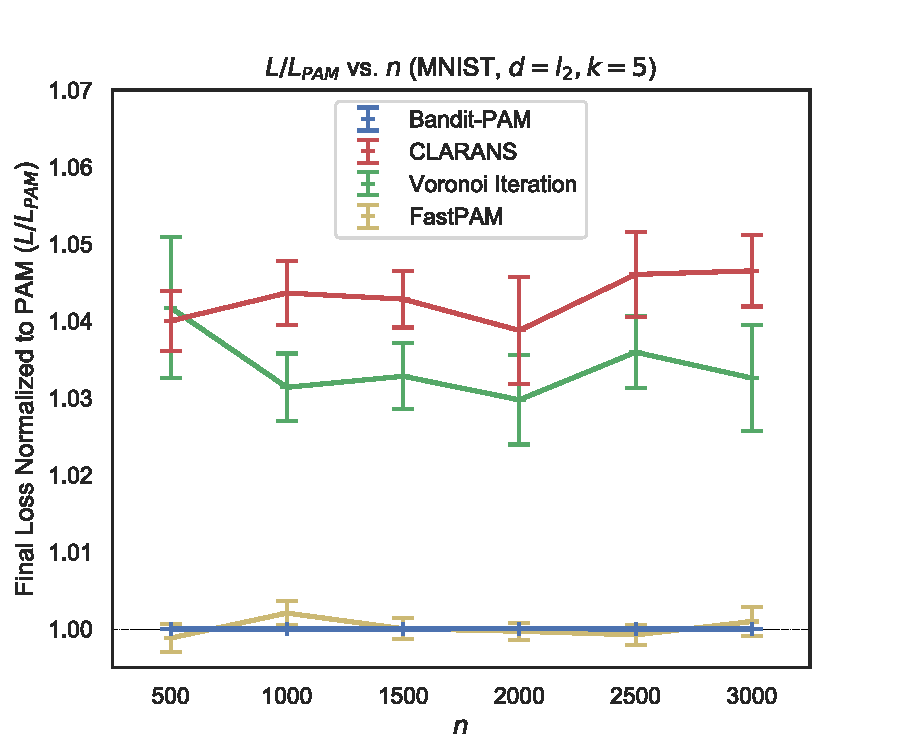
\includegraphics[width=\linewidth]{figures/loss_plot.pdf} 
        \caption{}
    \end{subfigure}
    \begin{subfigure}{.3\textwidth}
      \centering
      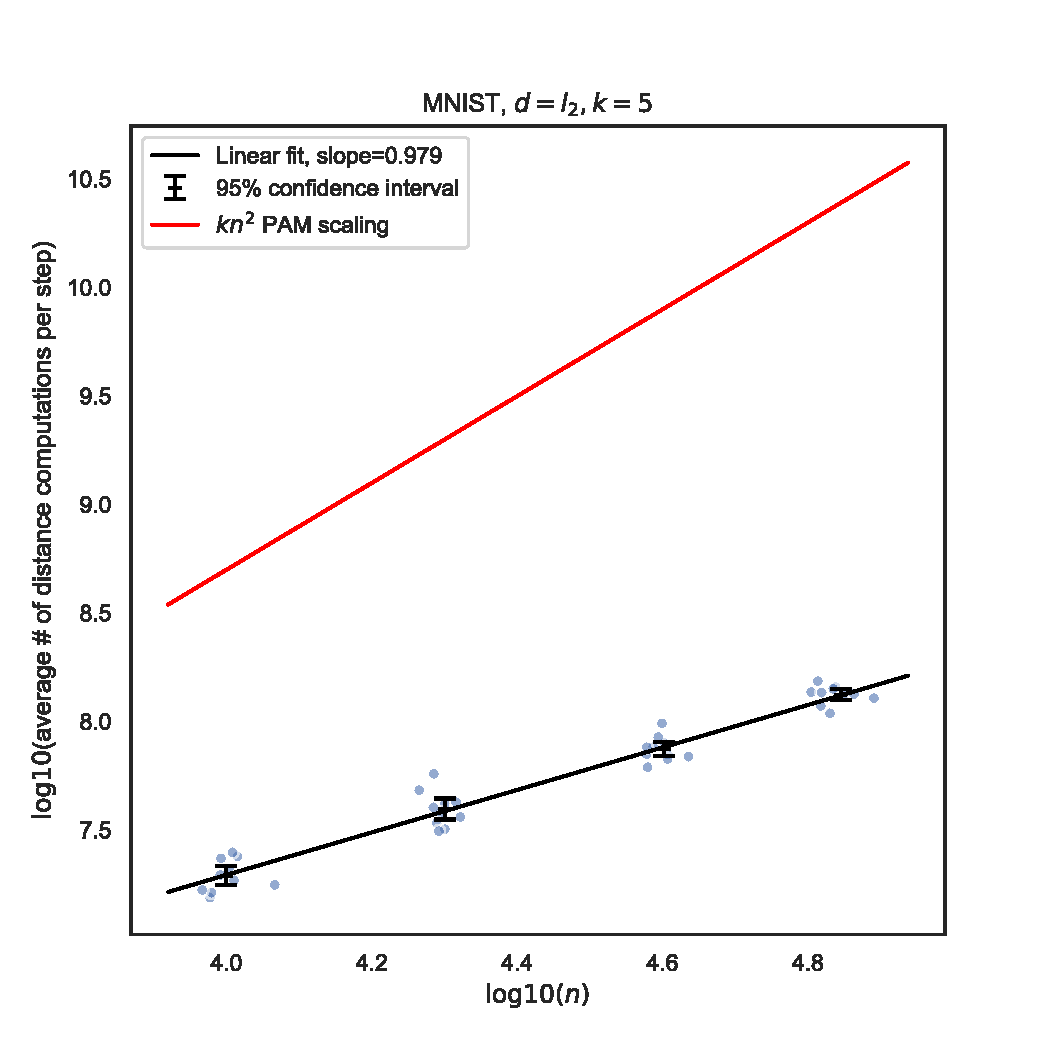
\includegraphics[width=\linewidth]{figures/MNIST-L2-k5.pdf}  
      \caption{}
    %   \label{fig:mods1}
    \end{subfigure}
    \begin{subfigure}{.3\textwidth}
      \centering
      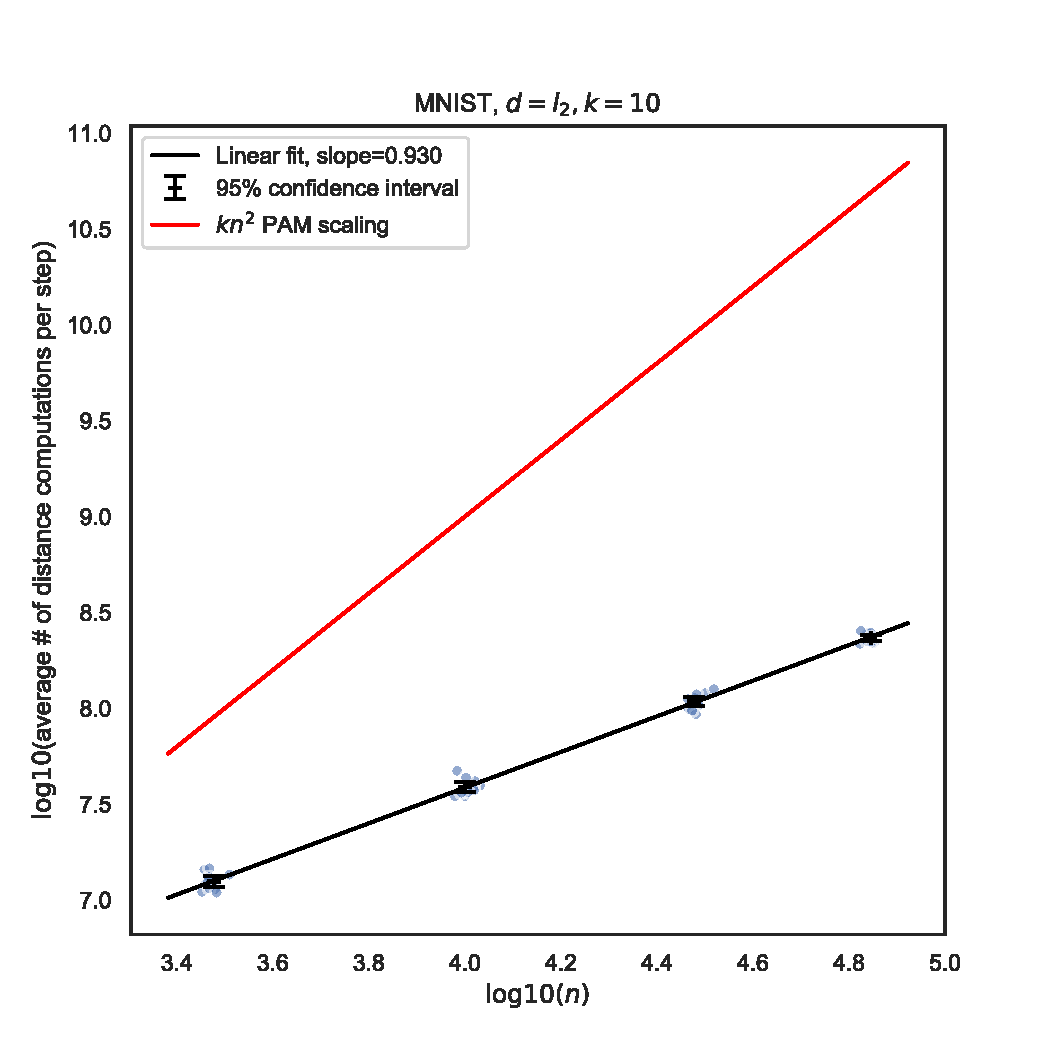
\includegraphics[width=\linewidth]{figures/MNIST-L2-k10.pdf}   
      \caption{}
    %   \label{fig:mods2}
    \end{subfigure}
    \caption{(a) Clustering loss relative to the PAM loss. Data is subsampled from MNIST, sample size $n$ varies from $500$ to $3000$, $k = 5$ and 95\% confidence intervals are provided. \algname always returns the same solution as PAM and hence has loss ratio $1$. FastPAM has a comparable performance, while the other two algorithms are significantly worse. 
    (b-c) Average number of distance calls per iteration vs sample size $n$ for MNIST and $l_2$ distance with (b) $k=5$ and (c) $k=10$. The plot is shown on a log-log scale. Lines of best fit (black) are plotted, as are reference lines demonstrating the expected scaling of PAM (red).}
    \label{fig:mods}
\end{figure}

\subsection{Clustering/loss quality \label{subsec:loss}}

%Baselines: PAM, CLARANS/CLARA, FastPAM, Voronoi Iteration
%The results from section \ref{Nscaling} show that each substep \algname scales almost linearly in dataset size. %Naturally, one might ask if there is a concession in final clustering quality that must be made for the $O(n/\log n)$ speedup of \algname. 

Figure \ref{fig:mods} (a) shows the relative losses of algorithms with respect to the loss of PAM. 
\algname and three other baselines, namely FastPAM \cite{schubert2019faster}, CLARANS \cite{ng2002clarans}, and Voronoi Iteration \cite{park2009simple}. 
We note that FastPAM is different from the FastPAM1 mentioned before; FastPAM takes $O(n^2)$ for each SWAP step but does not guarantee the same solution as PAM. 
\algname always returns the same solution as PAM and hence has loss ratio $1$. FastPAM has a comparable performance, while the other two algorithms are significantly worse. 

% normalized to the loss of PAM for various random subsets of MNIST.
% We observe that \algname finds solutions of equivalent quality to PAM, as does FastPAM, and that these solutions are better than the other baselines. 
% Indeed, in 59 of the 60 experiments, \algname tracks the exact optimization path and returns the exact same results as PAM; the single discrepancy arises in a single SWAP iteration of several hundred, which is in line with our choice of $\delta$.


% \algname always returns the same solution as PAM and hence has loss ratio $1$. FastPAM has a comparable performance, while the other two algorithms are significantly worse. 

% \mo{Need to describe hyperparameters for CLARANS?}


\subsection{Scaling with \texorpdfstring{$n$}{Lg} for different datasets, distance metric, and \texorpdfstring{$k$}{Lg} values \label{subsec:scaling}}

\begin{figure}[ht]
\begin{subfigure}{.33\textwidth}
  \centering
  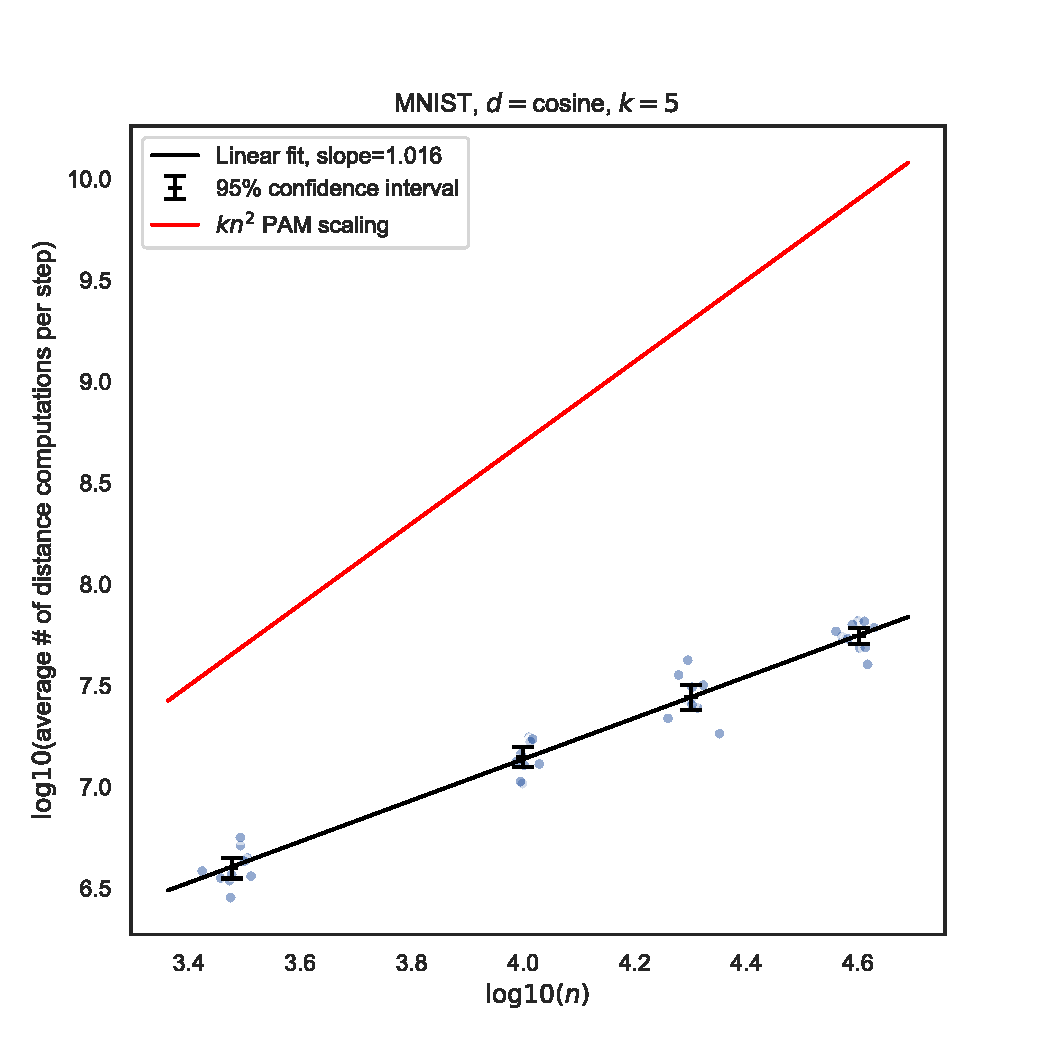
\includegraphics[width=\linewidth]{figures/MNIST-cosine-k5.pdf}  
  \caption{}
  \label{fig:scaling1}
\end{subfigure}
\begin{subfigure}{.33\textwidth}
  \centering
  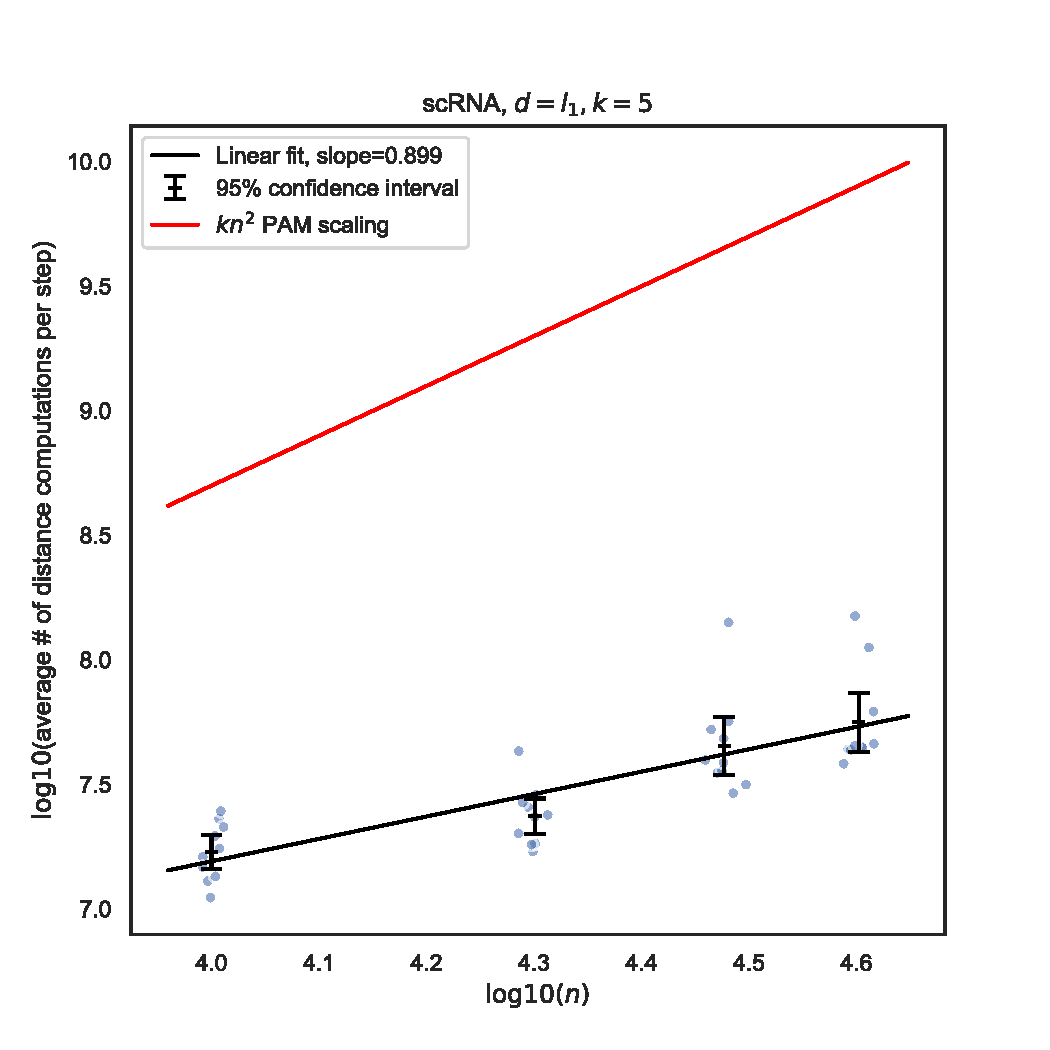
\includegraphics[width=\linewidth]{figures/SCRNA-L1-k5.pdf}   
  \caption{}
  \label{fig:scaling2}
\end{subfigure}
\begin{subfigure}{.33\textwidth}
  \centering
  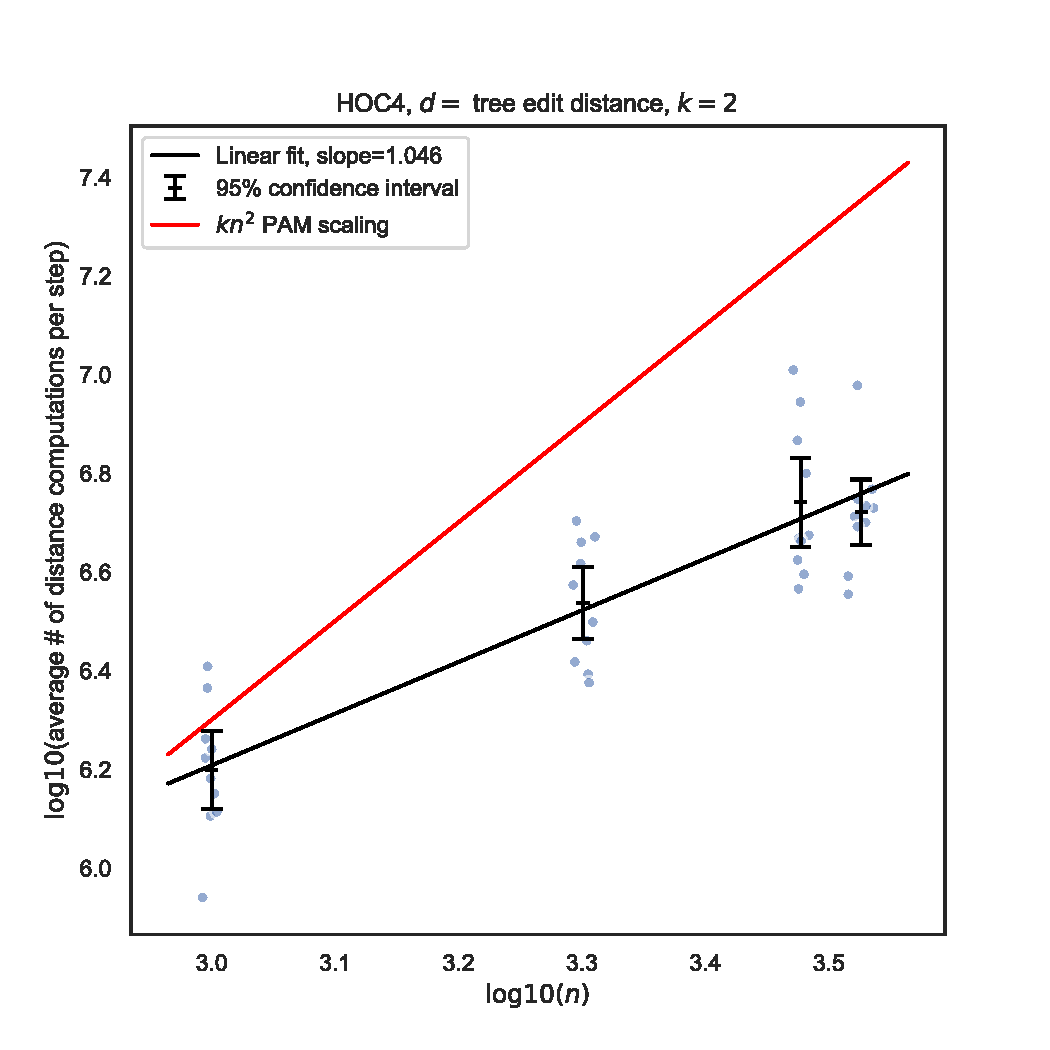
\includegraphics[width=\linewidth]{figures/HOC4-tree-k2.pdf}   
  \caption{}
  \label{fig:scaling3}
\end{subfigure}
\caption{Average number of distance calls per iteration vs sample size $n$, for (a) MNIST and cosine distance, (b) scRNA-seq and $l_1$ distance, and (c) HOC4 and tree edit distance. The plot is shown on a log-log scale. Lines of best fit (black) are plotted, as are reference lines demonstrating the expected scaling of PAM (red).}
\label{fig:scaling}
\end{figure}

%When assessing the scaling of \algnamenospace, we treat the entire BUILD step as a single SWAP iteration. Indeed, the entire BUILD procedure for the $k$-medoids problem on dataset $\mathcal{X}$ can be reduced to a single SWAP iteration for the $k+1$-medoids problem on the dataset $\mathcal{X}$ augmented with $k+1$ equal points infinitely far away from $\mathcal{X}$.

We next consider the number of distance calls per iteration as the sample size increases. 
The number of distance calls per iteration is defined as the total distance calls divided by the number of SWAP steps plus 1, where the plus 1 corresponds to the BUILD step. We choose to look at this quantity to account for different number of SWAPs for different runs, in order to provide a fair comparison. 

If the complexity is linear, then the slope would be $1$ in the log-log plot. 
Indeed, as shown in Figure \ref{fig:mods} (b-c), the slope for $k=5$ and $k=10$ are 0.979 and 0.930, respectively, indicating the scaling is linear in $n$ for different values of $k$. 

In addition, as shown in Figure \ref{fig:scaling}, the slopes of the log-log plot are 1.018, 0.899 and 1.046 for MNIST with cosine distance, scRNA-seq with $l_1$ distance, and HOC4 with tree edit distance, respectively, validating our theory that \algname takes almost linear number of distance evaluations per iteration for different datasets and different distance metrics.

% \subsection{Different distance metrics and increasing $k$ \label{subsec:mods}}

% Naturally, one might ask if \algname only demonstrates the expected speedup for a particular choice of metric for a given dataset. Figure \ref{fig:fig1} shows the scaling of the average number of distance calls in the BUILD step (Algorithm 1) and SWAP step (Algorithm 2) of \algname with $n$ for the MNIST dataset, but using cosine distance instead of $l_2$. \algname still runs in near-linear time; the slopes of the lines of best fit is 1.2 in BUILD and 1.1 in SWAP. These results suggest the algorithmic speedup of \algname is not dependence on the choice of distance metric used for a given dataset.

% Empirically, we observe that \algname exhibits almost-linear scaling for various choices of distance metric, even for the same dataset. Whereas Figure \ref{fig:scaling} (left) suggested that \algname scales linearly on MNIST when using cosine distance, Figure \ref{fig:mods} (left) suggests that \algname also scales linearly when considering $l_2$ distance on MNIST; the slope of the line of best fit is 0.979. 


% Additionally, we find that the scaling of \algname is not too sensitive to $k$, as long as $k \ll n$. Figure \ref{fig:mods} (right) demonstrates the scaling of \algname when $k$ is increased to 10; the slope of the line of best fit (0.930) still suggests roughly linear scaling in $n$.

%\mo{Mo: Add plots for MNIST,L2 k = 10 too}



% !TEX root = 0-main.tex

\section{Discussion and Conclusions}
\label{sec:discussion}

In all experiments, we have observed that the numbers of SWAPs are very small, typically fewer than 10, justifying the assumption of having an upper limit on the PAM SWAP step prior to running the algorithm in Sec. \ref{sec:theory}.   

We also observe that for all datasets, the randomly sampled distances have an empirical distribution similar to Gaussian distribution (Appendix Figures \ref{fig:sigma_ex_MNIST}-\ref{fig:sigma_ex_SCRNAPCA}), justifying the sub-Gaussian assumption in Sec. \ref{sec:theory}.
In addition, we observe that the the sub-Gaussian parameters are different for different steps and different points (Appendix Figures \ref{fig:MNIST_sigmas_example}), justifying the adaptive estimation of the sub-Gaussianity parameters in SubSec. \ref{subsec:algdetails}.

In addition, the distribution of the true arm parameters also mostly have a heavy-tailed distribution (Appendix Figure \ref{fig:mu_dist}), justifying the distributional assumption of $\mu_i$'s in Sec. \ref{sec:theory}. 

% We consider two different settings for each dataset. The first setting is that in which UltraPAM must return the same results as PAM. In this setting, we find that UltraPAM demonstrates significant algorithmic speedups over PAM, while returning the same results with high probability. In the second setting, we relax this requirement that UltraPAM returns the same results as PAM. In the latter setting, we find that UltraPAM demonstrates an even greater speedup over PAM, while finding final medoid assignments that are nearly the same quality as those found by PAM and occasionally even better.

% \textbf{Applications and Impact:}  

% We provide opportunities for future work in Appendix \ref{sec:future}.

Our application to the HOC4 dataset also suggests a method for scaling personalized feedback to individual students in online courses. If limited resources are available, instructors can choose to provide feedback on just the \textit{medoids} of submitted solutions instead of exhaustively providing feedback on \textit{every} unique solution, of which there may be several thousand. Instructors can then refer individual students to the feedback provided for their closest medoid. We anticipate that this approach can be applied generally for students of Massive Open Online Courses (MOOCs), thereby enabling more equitable access to education and personalized feedback for students.

% !TEX root = 0-main.tex

\section*{Broader Impact}
\label{sec:impact}

In this work, we proposed an algorithm that accelerated finding solutions to the $k$-medoids problem while producing comparable -- and usually equivalent -- final cluster assignments. Our work enables the discovery of high-quality medoid assignments in very large datasets, including some on which prior algorithms were prohibitively expensive. A potential negative consequence of this is that practitioners may be incentivized to gather and store larger amounts of data now that it can be meaningfully processed, in a phenomenon more generally described as induced demand \cite{induceddemand}. This incentive realignment could potentially result in negative externalities such as an increase in energy consumption and carbon footprints.

We also anticipate, however, that \algname will enable several beneficial applications in biomedicine, education, and fairness. For example, the evolutionary pathways of infectious diseases could possibly be constructed from the medoids of genetic sequences available at a given point in time, if prior temporal information about these sequences' histories is not available. Similarly, the medoids of patients infected in a disease outbreak may elucidate the origins of outbreaks, as did prior analyses of cholera outbreaks using Voronoi Iteration \cite{cholera}. As discussed in Section \ref{sec:discussion}, our application to the HOC4 data also demonstrates the utility of \algname in online education. In particular, especially with recent interest in online learning, we hope that our work will improve the quality of online learning for students worldwide.


% \begin{ack}
% \label{ack}
% My mom, and \cite{kaufman1990partitioning} for natbib
% \end{ack}

\bibliographystyle{plain}
\bibliography{refs}

% !TEX root = 0-main.tex

\clearpage
\section*{Appendix}
\label{appendix}

\renewcommand\thefigure{\arabic{figure}}
\setcounter{figure}{1}      
\setcounter{section}{0}      

\renewcommand{\figurename}{Appendix Figure}

\section{Additional Discussions}
\subsection{FastPAM1 optimization}
\label{A2}

Algorithm \ref{alg:bandit_based_search} can also be combined with the FastPAM1 optimization from \cite{schubert2019faster} to reduce the number of computations in each SWAP iteration. 
For a given candidate swap $(m, x)$, we rewrite $g_{(m,x)}(x_j)$ from Eq. \eqref{eqn:swap_instance} as:
\begin{equation}
    \label{eqn:fastpam1-trick}
    g_{m,x}(x_j) = - d_1(x_j) + \mathbbm{1}_{x_j \notin \mathcal{C}_m}\min[d_1(x_j),d(x,x_j)] + \mathbbm{1}_{x_j \in \mathcal{C}_m}\min[d_2(x_j), d(x, x_j)]
\end{equation}
where $\mathcal{C}_m$ denotes the set of points whose closest medoid is $m$ and $d_1(x_j)$ and $d_2(x_j)$ are the distance from $x_j$ to its nearest and second nearest medoid, respectively, before the swap is performed. 
We cache the values $d_1(x_j), d_2(x_j)$, and the cluster assignments $\mathcal{C}_m$ so that Eq. \eqref{eqn:fastpam1-trick} no longer depends on $m$ and instead depend only on $\mathbbm{1}_{\{x_j \in \mathcal{C}_m \}}$, which is cached. This allows for an $O(k)$ speedup in each SWAP iteration since we do not need to recompute Equation \ref{eqn:fastpam1-trick} for each of the $k$ distinct medoids ($m$s).


\subsection{Value of re-estimating each \texorpdfstring{$\sigma_x$}{Lg}}
\label{A1}

% Allowing for arm-dependent $\sigma_x$ and re-estimating each $\sigma_x$ in each iteration also presents a difference between our approach and prior work {\bf \{citation\}}. Details about these techniques are discussed further in Section \ref{exps}. 


% We make the following additional changes to the vanilla version of Algorithm \ref{alg:bandit_based_search} to further improve speed. 

% The parameter $\sigma_x$ for the confidence intervals are estimated from data. Specifically, %\martin{Mo: could you add more information?}.
% We found that having different parameters for different steps of PAM will greatly improve speed. 
% We also found that the speed can be further improved by allowing a different parameter for different target points in $\mathcal{S}_{\text{tar}}$. 
% \martin{(As demonstrated in ...)}

\begin{figure}[h!]
    \centering
    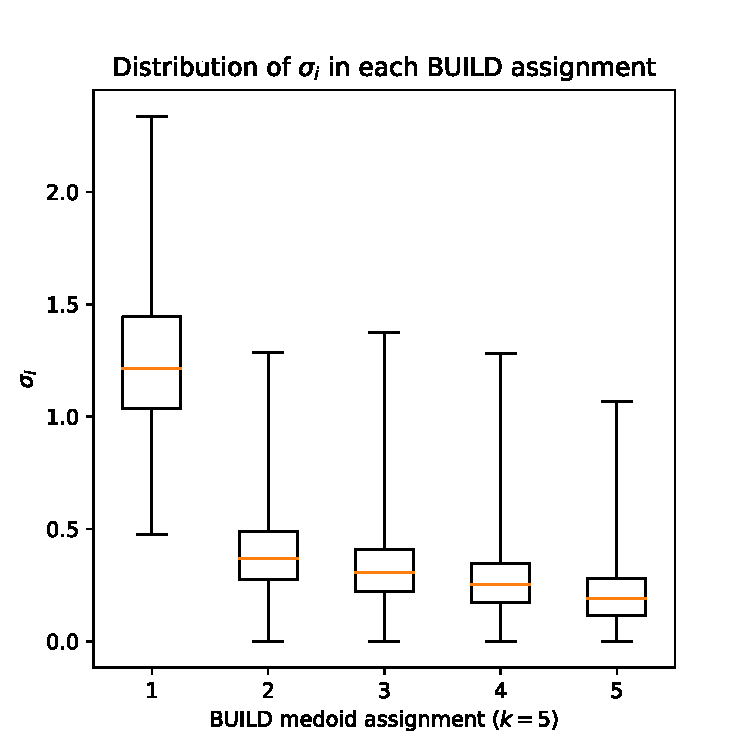
\includegraphics[scale=0.5]{figures/MNIST_sigmas_example.pdf}
    \caption{Boxplot showing the min, max, and each quartile for the set of all $\sigma_x$ estimates for the full MNIST dataset, in the BUILD step. } 
    \label{fig:MNIST_sigmas_example}
\end{figure}

The theoretical results in Section \ref{sec:theory} and empirical results in Section \ref{sec:exps} suggest that \algname scales almost linearly in dataset size for a variety of real-world datasets and commonly used metrics. One may also ask if Lines 7-8 of Algorithm \ref{alg:bandit_based_search}, in which we re-estimate each $\sigma_i$ from the data, are necessary.
In some sense, we treat the set of \{$\sigma_i$\} as adaptive in two different ways: $\sigma_i$ is calculated on a \textit{per-arm} basis (hence the subscript $i$), as well recalculated in each BUILD and SWAP iteration.
In practice, we observe that re-estimating each $\sigma_x$ for each sequential call to Algorithm \ref{alg:bandit_based_search} significantly improves the performance of our algorithm. Figure \ref{fig:MNIST_sigmas_example} describes the distribution of estimate $\sigma_x$ for the MNIST data at different stages of the BUILD step. The median $\sigma_x$ drops dramatically after the first medoid has been assigned and then steadily decreases, as indicated by the orange lines, and suggests that each $\sigma_x$ should be recalculated at every assignment step. Furthermore, the whiskers demonstrate significant variation amongst the $\sigma_x$ in a given assignment step and suggest that having arm-dependent $\sigma_x$ parameters is necessary. Without these modifications to our algorithm, we find that the confidence intervals used by \algname (Line 8) are unnecessarily large and cause computation to be expended needlessly as it becomes harder to identify good arms. Intuitively, this is due to the much larger confidence intervals that make it harder to distinguish between arms' mean returns.
For a more detailed discussion of the distribution of $\sigma_x$ and examples where the assumptions of Theorem \ref{thm:nlogn} are violated, we refer the reader to Appendix \ref{A3}.



\subsection{Violation of distributional assumptions}
\label{A3}

In this section, we investigate the robustness of \algname to violations of the assumptions in Theorem \ref{thm:nlogn} on an example dataset and provide intuitive insights into the degradation of scaling. We create a new dataset from the scRNA dataset by projecting each point onto the top 10 principal components of the dataset; we call the dataset of projected points scRNA-PCA. Such a transformation is commonly used in prior work; the most commonly used distance metric between points is then the $l_2$ distance \cite{scrnabestpractices}.

Figure \ref{fig:mu_dist} shows the distribution of arm parameters for various (dataset, metric) pairs in the first BUILD step. In this step, the arm parameter corresponds to the mean distance from the point (the arm) to every other point. We note that the true arm parameters in scRNA-PCA are more heavily concentrated about the minimum than in the other datasets. Intuitively, we have projected the points from a 10,170-dimensional space into a 10-dimensional one and have lost significant information in doing so. This makes many points appear "similar" in the projected space.

Figures \ref{fig:sigma_ex_MNIST} and \ref{fig:sigma_ex_SCRNAPCA} show the distribution of arm rewards for 4 arms (points) in MNIST and scRNA-PCA, respectively, in the first BUILD step. We note that the examples from scRNA-PCA display much larger tails, suggesting that their sub-Gaussianity parameters $\sigma_x$ are very high.

Together, these observations suggest that the scRNA-PCA dataset may violate the assumptions of Theorems \ref{thm:nlogn} and \ref{thm:specific} and hurt the scaling of \algname with $n$. Figure \ref{fig:SCRNAPCA-L2-scaling} demonstrates the scaling of \algname with $n$ on scRNA-PCA. The slope of the line of best fit is 1.204, suggesting that \algname scales as approximately $O(n^{1.2})$ in dataset size. We note that this is higher than the exponents suggested for other datasets by Figures \ref{fig:mods} and \ref{fig:scaling}, likely to the different distributional characteristics of the arm means and their spreads.

We note that, in general, it may be possible to characterize the distribution of arm returns $\mu_i$ at and the distribution of $\sigma_x$, the sub-Gaussianity parameter, at every step of \algnamenospace, from properties of the data-generating distribution, as done for several distributions in \cite{bagaria2018medoids}. We leave this more general problem, as well as its implications for the complexity of our \algname, to future work.

\begin{figure}[ht]
\begin{subfigure}{.5\textwidth}
  \centering
  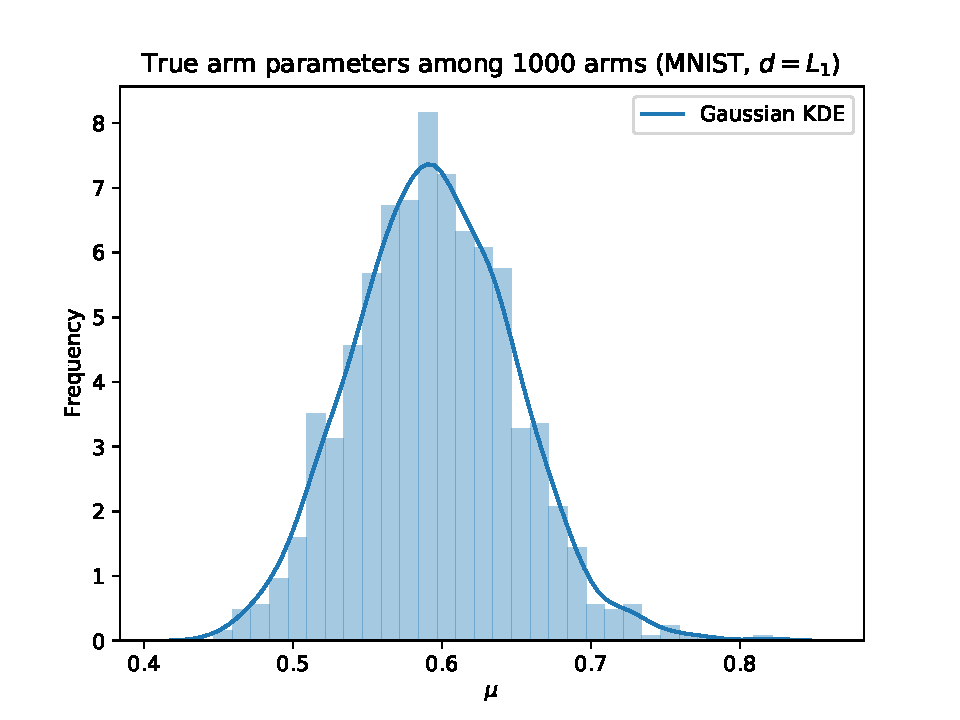
\includegraphics[width=\linewidth]{figures/mu-MNIST-COSINE.pdf}  
  \label{fig:mu_dist1}
\end{subfigure}
\begin{subfigure}{.5\textwidth}
  \centering
  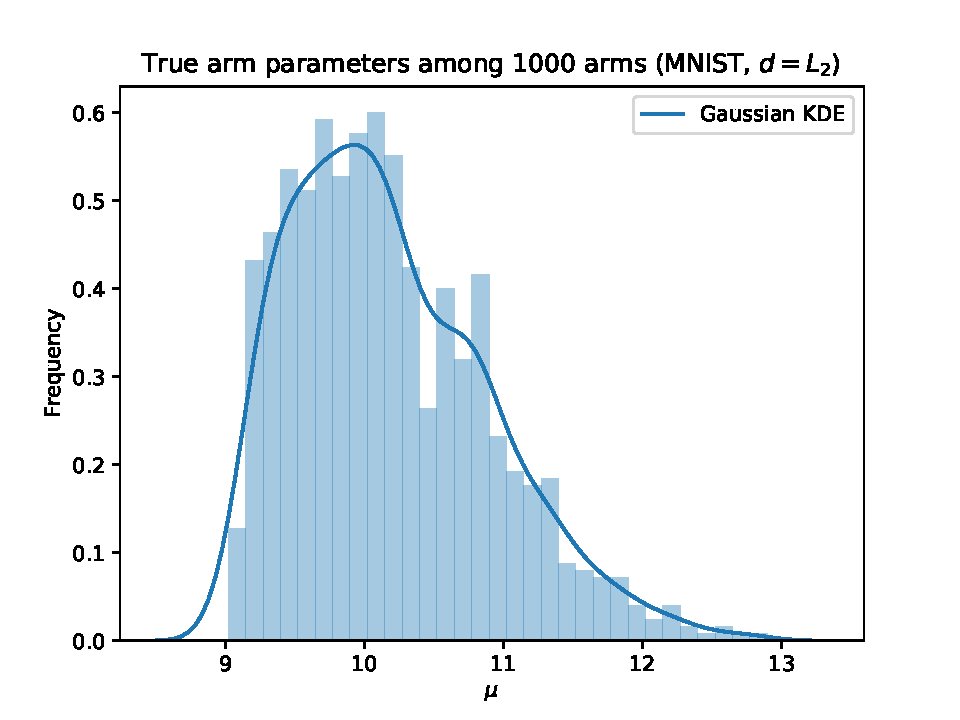
\includegraphics[width=\linewidth]{figures/mu-MNIST-L2.pdf}   
  \label{fig:mu_dist2}
\end{subfigure}
\begin{subfigure}{.5\textwidth}
  \centering
  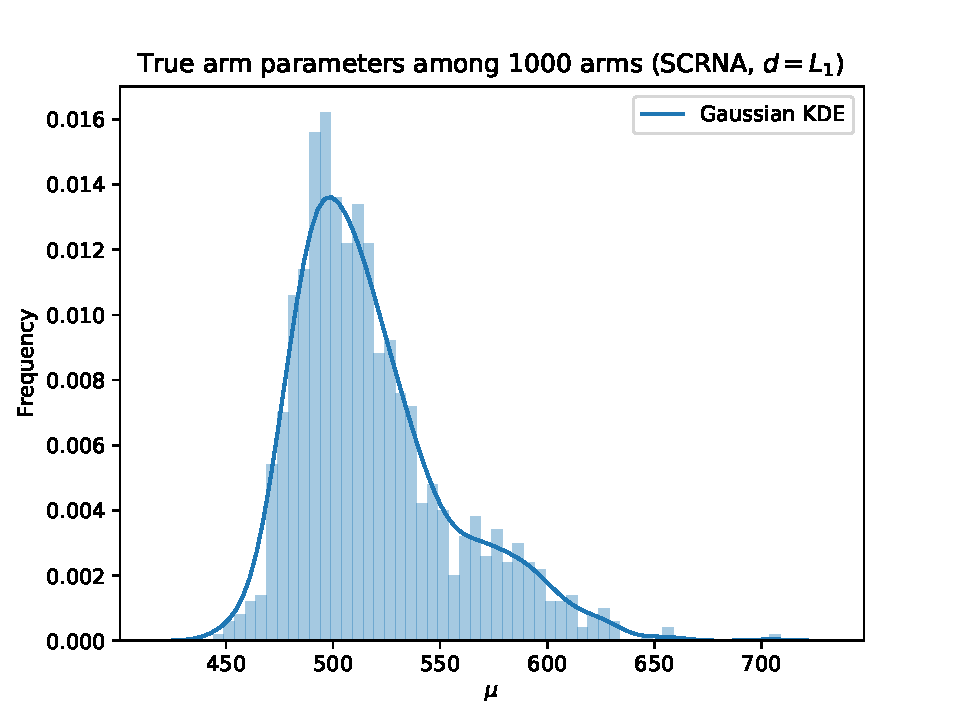
\includegraphics[width=\linewidth]{figures/mu-SCRNA-L1.pdf}   
  \label{fig:mu_dist3}
\end{subfigure}
\begin{subfigure}{.5\textwidth}
  \centering
  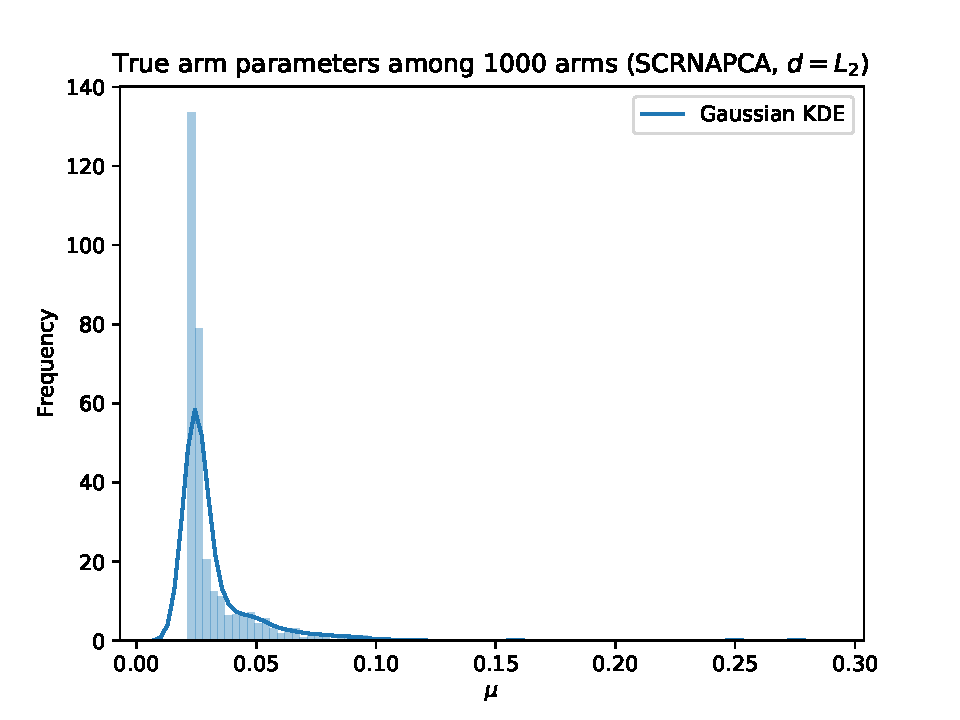
\includegraphics[width=\linewidth]{figures/mu-SCRNAPCA-L2.pdf}   
  \label{fig:mu_dist4}
\end{subfigure}
\caption{Histogram of true arm parameters, $\mu_i$, for 1000 randomly sampled arms in the first BUILD step of various datasets. For scRNA-PCA with $d = l_2$ (bottom right), the arm returns are much more sharply peaked about the mininum than for the other datasets. In plots where the bin widths are less than 1, the frequencies can be greater than 1.}
\label{fig:mu_dist}
\end{figure}

\begin{figure}[ht]
\begin{subfigure}{.5\textwidth}
  \centering
  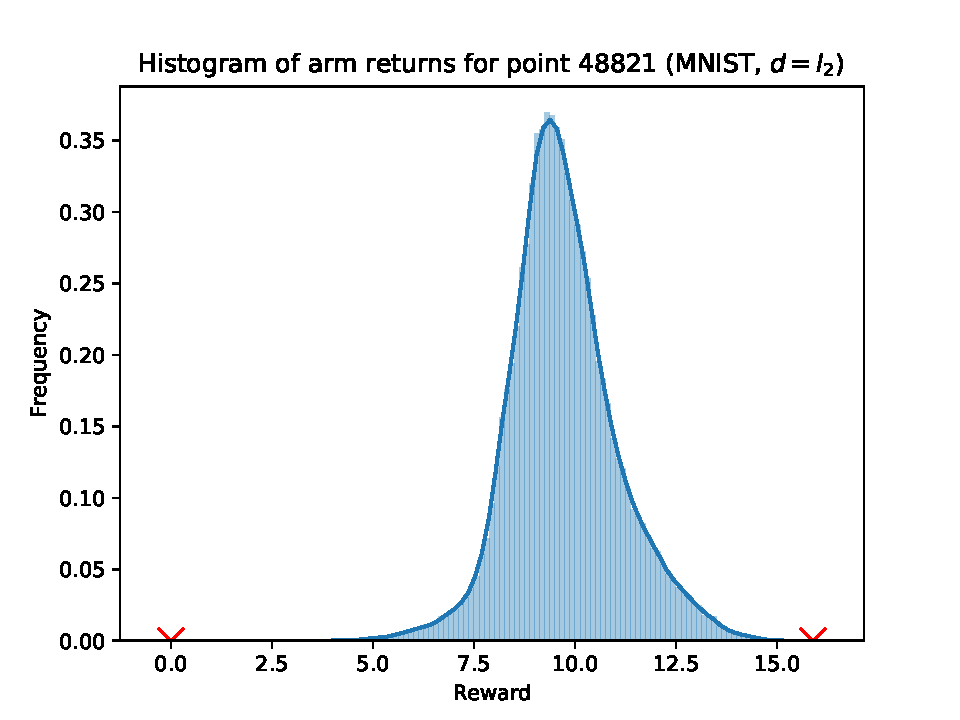
\includegraphics[width=\linewidth]{figures/sigma-MNIST-0-L2.pdf}  
\end{subfigure}
\begin{subfigure}{.5\textwidth}
  \centering
  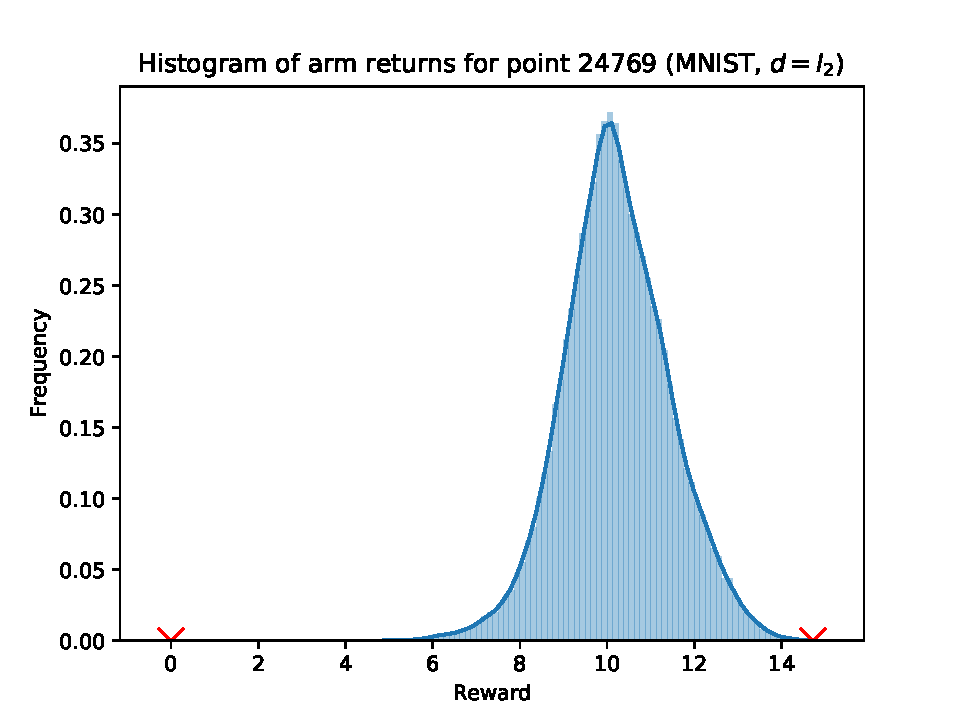
\includegraphics[width=\linewidth]{figures/sigma-MNIST-1-L2.pdf}   
\end{subfigure}
\begin{subfigure}{.5\textwidth}
  \centering
  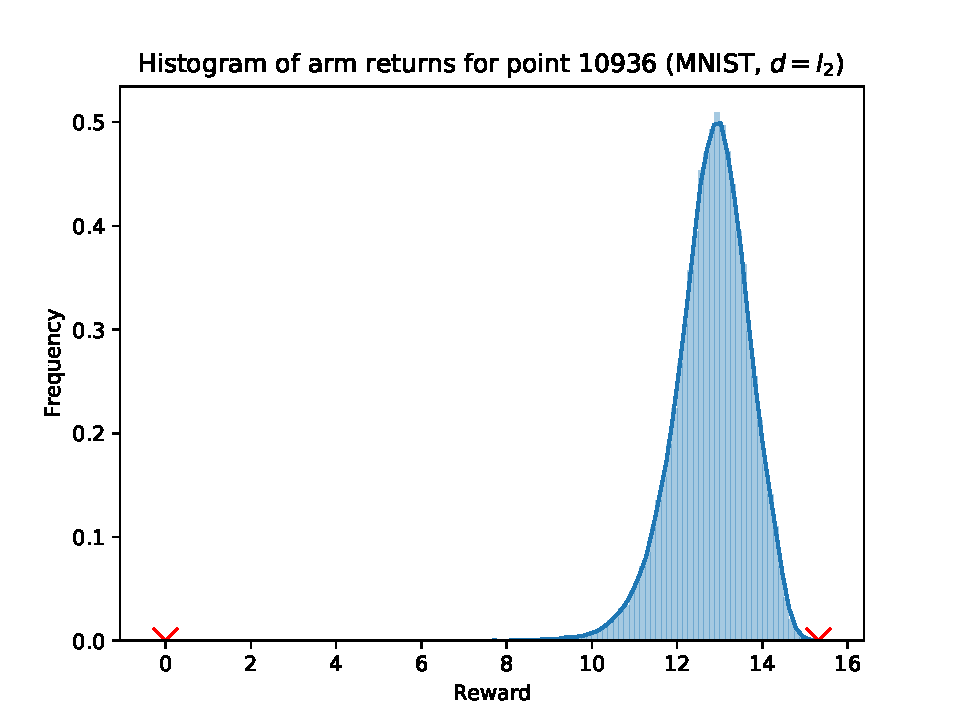
\includegraphics[width=\linewidth]{figures/sigma-MNIST-2-L2.pdf}   
\end{subfigure}
\begin{subfigure}{.5\textwidth}
  \centering
  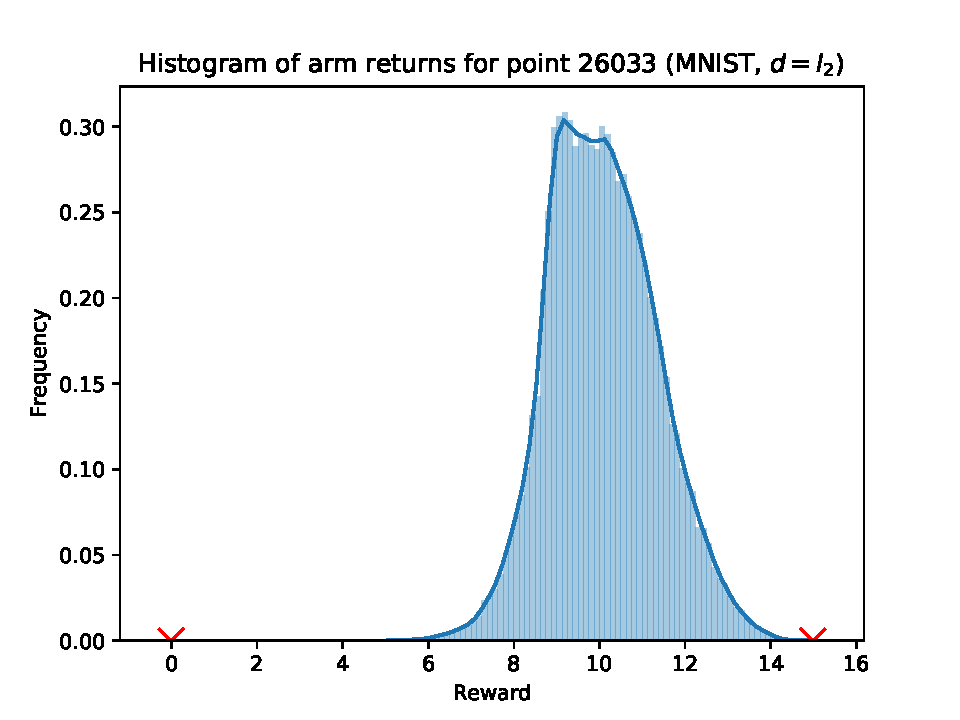
\includegraphics[width=\linewidth]{figures/sigma-MNIST-3-L2.pdf}   
\end{subfigure}
\caption{Example distribution of rewards for 4 points in MNIST in the first BUILD step. The minimums and maximums are indicated with red markers.}
\label{fig:sigma_ex_MNIST}
\end{figure}


\begin{figure}[ht]
\begin{subfigure}{.5\textwidth}
  \centering
  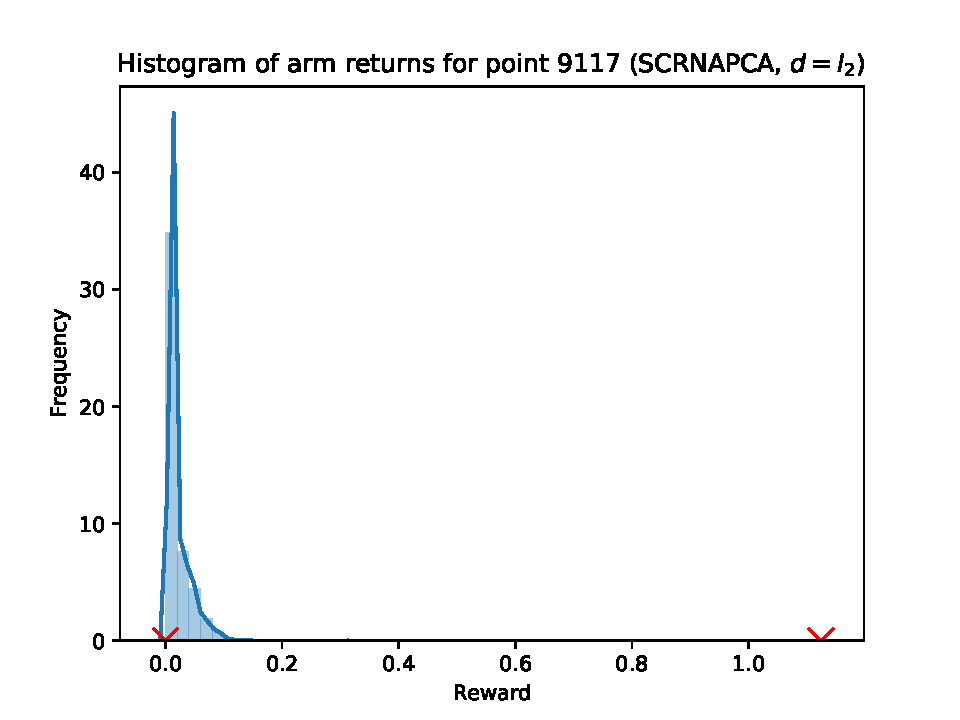
\includegraphics[width=\linewidth]{figures/sigma-SCRNAPCA-0-L2.pdf}  
\end{subfigure}
\begin{subfigure}{.5\textwidth}
  \centering
  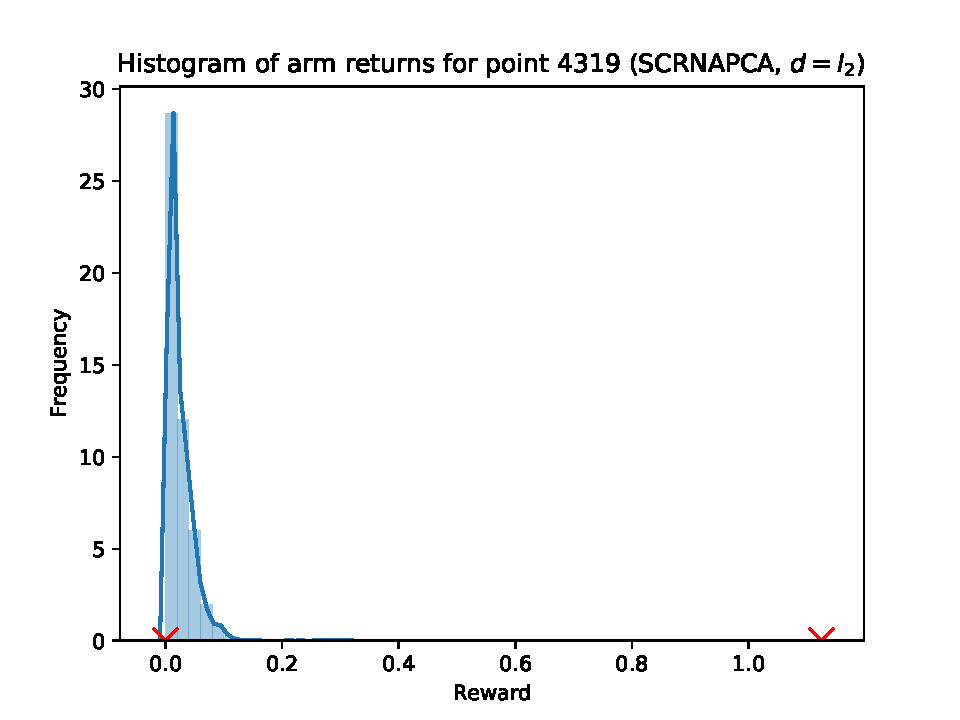
\includegraphics[width=\linewidth]{figures/sigma-SCRNAPCA-1-L2.pdf}   
\end{subfigure}
\begin{subfigure}{.5\textwidth}
  \centering
  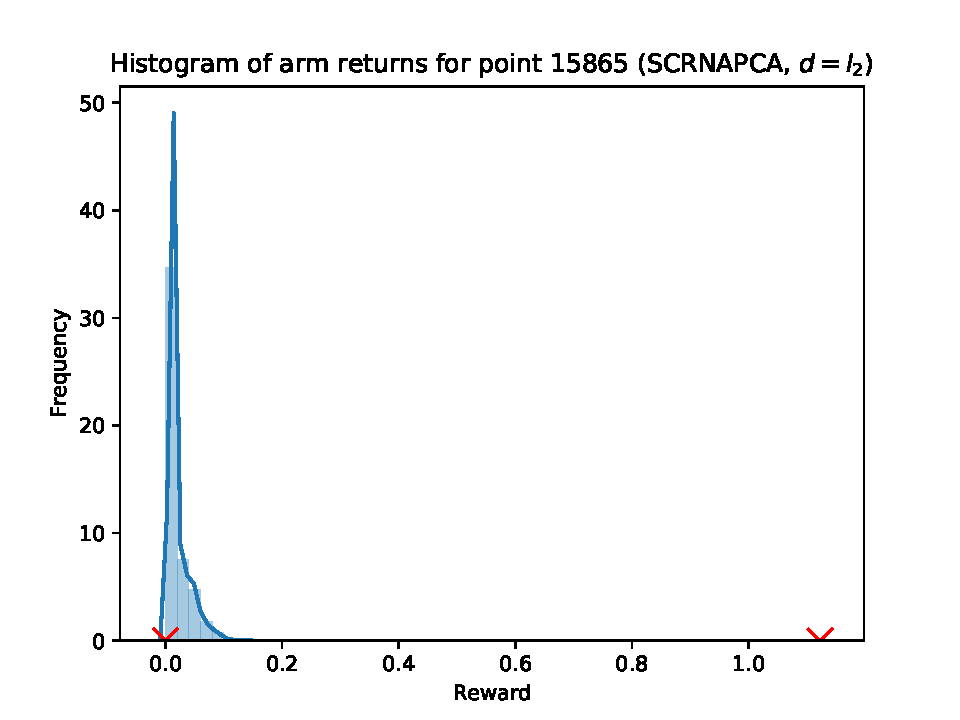
\includegraphics[width=\linewidth]{figures/sigma-SCRNAPCA-2-L2.pdf}   
\end{subfigure}
\begin{subfigure}{.5\textwidth}
  \centering
  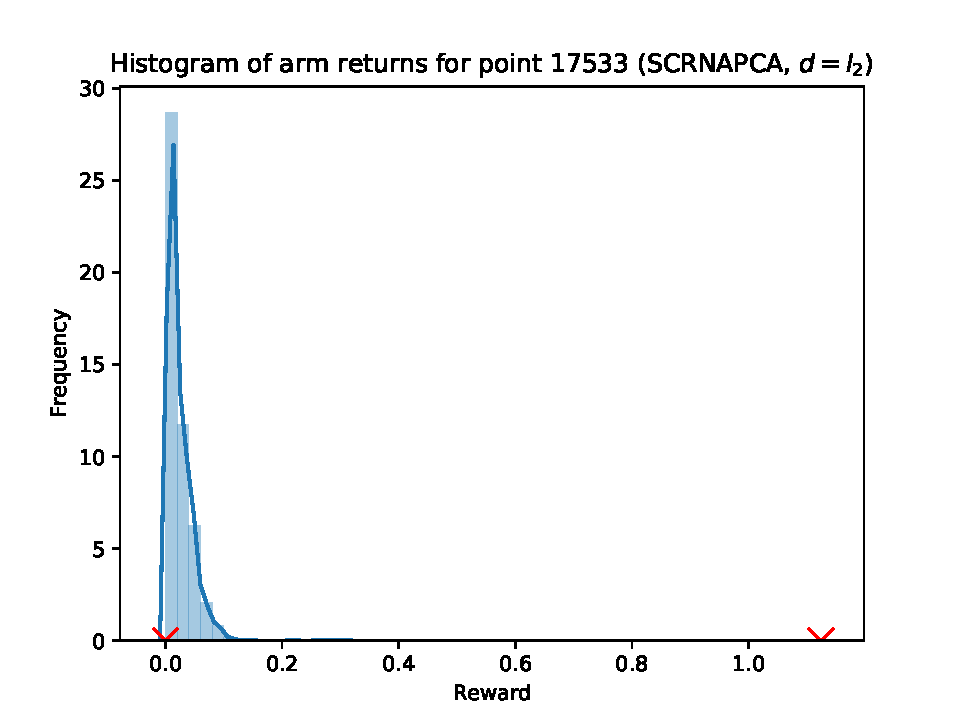
\includegraphics[width=\linewidth]{figures/sigma-SCRNAPCA-3-L2.pdf}   
\end{subfigure}
\caption{Example distribution of rewards for 4 points in scRNA-PCA in the first BUILD step. The minimums and maximums are indicated with red markers. The distributions shown here are more heavy-tailed than in Figure \ref{fig:sigma_ex_MNIST}. In plots where the bin widths are less than 1, the frequencies can be greater than 1.}
\label{fig:sigma_ex_SCRNAPCA}
\end{figure}


\begin{figure}[ht!]
    \centering
    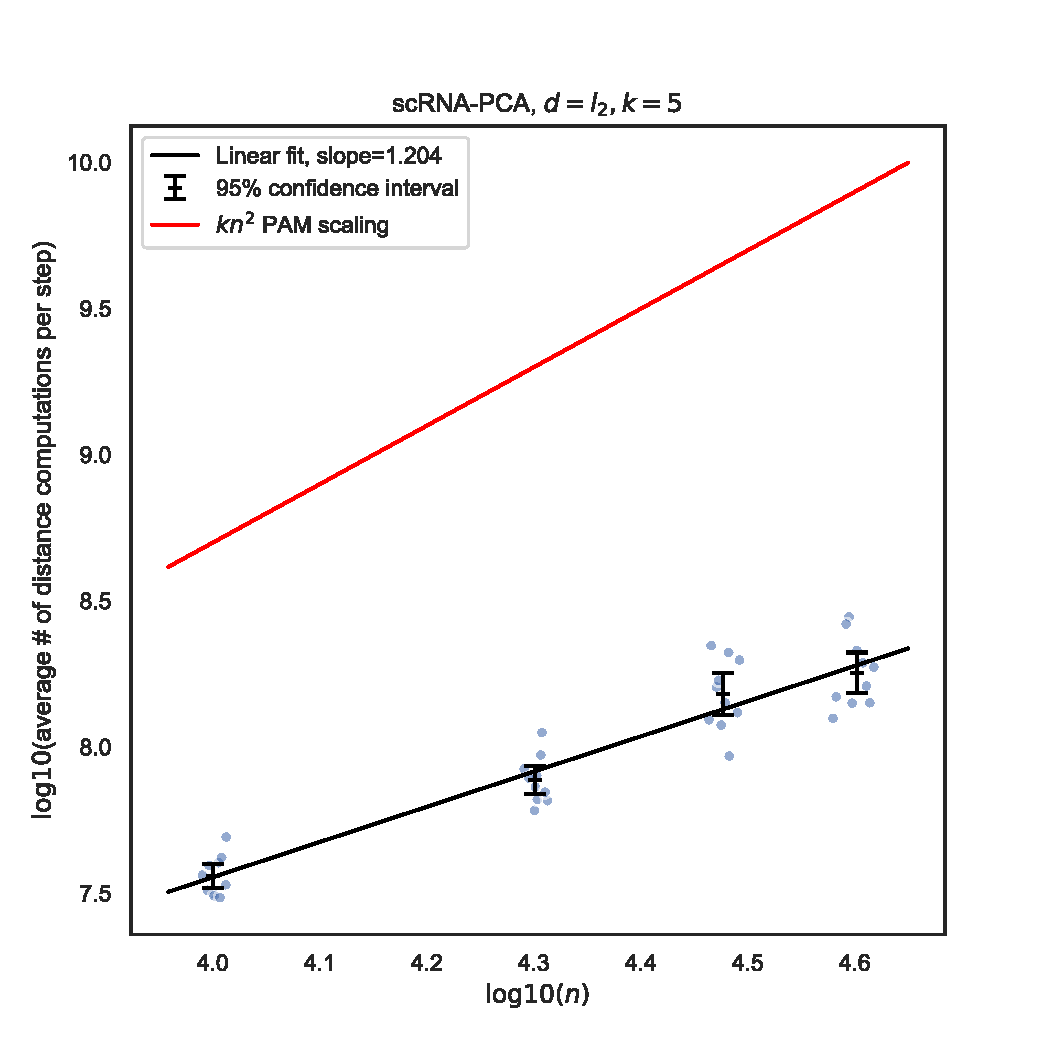
\includegraphics[scale=0.5]{figures/SCRNAPCA-L2-k5.pdf}
    \caption{Average number of distance calls per iteration vs $n$, for scRNA-PCA and $l_2$ distance on a log-log scale. The line of best fit (black) are plotted, as are reference lines demonstrating the expected scaling of PAM (red).} 
    \label{fig:SCRNAPCA-L2-scaling}
\end{figure}

\newpage
\clearpage
\section{Future Work}
\label{sec:future}
% \martin{Maybe move this section to Appendix}

% As part of this work, we developed and released a Python implementation of \algname. The runtime of our algorithms, as measured by wall time, could be significantly improved by reimplementing the algorithm in C++. In the future, we intend to release a high-performance C++ library for MAB-Based $k$-medoids algorithms, which could also be called from Python. Though we do not the theoretical complexity of the algorithm to differ amongst different language implementations, we can expect as large as a 20x improvement in wall time by reimplementing the algorithm in C++ \{citation\}.

% We also note that the PAM algorithm is used widely as a subroutine in several downstream algorithms, such as CLARA and CLARANS \{citation\}. \algname can be used as a modular "swap-in" for PAM these other algorithms, and would improve those algorithms' theoretical complexities and running times.

There are several ways in which \algname could be improved or made more impactful. In this work, we chose to implement a UCB-based algorithm to find the medoids of a dataset. Other best-arm-identification approaches, however, could also be used for this problem. 
%In particular, Thompson sampling may offer improvements over the UCB algorithm used here \{citation\}. 
An alternate approach using bootstrap-based bandits could also be valuable, especially in relaxing the distributional assumptions on the data that the quantities of interest are $\sigma$-sub-Gaussian \cite{wang2020bootstrap, kveton2019abootstrap, kveton2019bbootstrap}. It may also be possible to generalize a recent single-medoid approach, Correlation-Based Sequential Halving \cite{baharav2019ultra}, to more than 1 medoid. Though we do not have reason to suspect an algorithmic speedup (as measured by big-O), we may see constant factor improvements or improvements in wall clock time.

Throughout this work, we assumed that computing the distance between two points was an $O(1)$ operation. This obfuscates the dependence on the dimensionality of the data, $d$. If we consider computing the distance between two points an $O(d)$ computation, the complexity of \algname could be expressed as $O(dn$log$n)$ in the BUILD step and each SWAP iteration. Recent work \cite{bagaria2018adaptive} suggests that this could be further improved; instead of computing the difference in each of the $d$ coordinates, we may be able to adaptively sample which of the $d$ coordinates to use in our distance computations and reduce the dependence on dimensionality from $d$ to $O(\log d)$, especially in the case of sparse data.
%We note, however, that in practice most libraries contain software optimizations that make the dependence on $d$ for a distance computation sublinear (e.g. architecture optimizations); as such, we did not consider implementing this optimization in our work. 

% It is also important to note that the dissimilarity function used in the loss computation (Equation 1) is not required to be a distance metric; an arbitrary, even asymmetric, dissimilarity function could be used in more general settings.

Finally, it may be possible to improve the theoretical bounds presented in Theorem 1. We also note that it may be possible to prove the optimality of \algname in regards to algorithmic complexity, up to constant factors, using techniques from \cite{bagaria2018medoids} that were developed for sample-efficiency guarantees in hypothesis testing.

%Indeed, in our experiments, we found that \algname results agreed with PAM results with far more liberal error probability thresholds, $\delta$, than that suggested by Theorem 1, which allowed for better wall times. In fact, it may be possible to learn the "optimal" implementation parameters, such as $\delta$ and $\sigma$, directly from the data instead of empirically estimating them and treating them as constants. 


% Notes: Assuming sigma-sub-Guassian at the first step implies sigma-sub-Gaussian for later medoids. Do proof for k = 1 first and then induction.

% Let ${X_1, X_2, ..., X_N}$ each be $\sigma$-sub-Gaussian variables. Then, at the termination of the UCB algorithm when a new medoid is selected [i.e. lowest confidence interval is disjoint from others], we have that, for each $\mu_i$, with probability $1 - \delta$, $\mu_i \in [\hat{\mu_i} - C_i(t), \hat{\mu_i} + C_i(t)]$, where $C_i(t) = \sqrt{\frac{2\sigma^2log\frac{2}{\delta}}{T_i(t)}}$. Thus, with probability at least $1 - kN\delta$, the BUILD step of the UCB-based UltraPAM returns the same result as the BUILD step of PAM. Furthermore, if the original PAM algorithm takes $T$ SWAP steps to converge, then with probability  at least $1 - Tk(N-k)\delta$, the SWAP step of UltraPAM returns the same result as PAM. 

% Proof: At the termination of a single medoid assignment of the UltraPAM build step, the lowest confidence interval must be disjoint from all the other confidence intervals. Let the true medoid be point $1$ In order for an error to be made, at the end of the sampling, either $\hat{\mu_1}$ must be outside of its confidence interval or some other point (that will be incorrectly be chosen as the medoid) must be outside of its confidence interval [if none of these were true, we would not have an error -- crux of the argument]. By union bounding over the probability of any $\hat{\mu_i}$ not being in its confidence interval, we have:

% $P($Error in single BUILD assignment$) \leq N\delta$

% By union bounding this over all $k$ BUILD assignments, we have

% $P($Error in all BUILD$) \leq kN\delta$

% Thus, with probability at least $1 - kN\delta$, the BUILD step of UltraPAM chooses the same initial $k$ medoids as PAM.

% Pf. Similar to above, but with $T$ iterations and $k(N-k)$ arms. So error is 

% $P($Error in all SWAP$) \leq Tk(N-k)\delta$



% Note: define consistency as agreeing with PAM.

% 1. Best-arm identification
% 2. Same results as PAM
% 3. Number of swap steps
% 4. Quantify how often fallback occurs


% % \begin{algorithm}[t]
% %   \caption{\texttt{Med-dit} \label{alg:UCB-Medoid}}
% %   \label{alg:cpca1}
% % \begin{algorithmic}[1]
% %   \STATE Evaluate 
% %   distances 
% %   of each point to a randomly 
% %   chosen point and build a $(1-\delta)$-confidence interval
% %   for the mean distance 
% %   of each point $i$:
% %   $[\hat{\mu}_i(1)-C_i(1), \ \hat{\mu}_i(1)+C_i(1)]$.    
% %   \WHILE \TRUE
% %   \STATE At iteration $t$, pick point $A_t$ that 
% %   minimises $\hat{\mu}_i(t-1)-C_i(t-1)$.    
% %     \IF{distances of point $A_t$ are 
% %   evaluated less than $n-1$ times}
% %     \STATE evaluate the distance
% %   of $A_t$ to a randomly picked point 
% %   and update the confidence interval of $A_t$.
% %     \ELSE
% %     \STATE Set 
% %   $\hat{\mu}_i(t)$ to be the empirical mean 
% %   of distances of point $A_t$ by 
% %   computing its distance to all $(n-1)$ other
% %   points and set 
% %   $C_{A_t}(t)=0$.
% %   \ENDIF
% %   \IF {there exists a point $x_{i^*}$ 
% %   such that $\forall  i\neq i^*$, 
% %   $\hat{\mu}_{i^*}(t) + C_{i^*}(t) < \hat{\mu}_i(t) - C_i(t)$}
% %     \RETURN $x_{i^*}$.
% %   \ENDIF  
% %   \ENDWHILE
% % \end{algorithmic}
% % \end{algorithm}




% %%% For use with ALGORITHMC package
% % \begin{algorithm}[t]
% % \caption{\texttt{UltraPAM\_BUILD($X, k_{max}, d$):} \label{alg:ultrapam-build}}

% % \begin{algorithmic}[1]
% %     \FOR{$k = 1, 2, ..., k_{max}$}
% %     \STATE $\mathcal{M} = \emptyset$
% %     \STATE $arms \leftarrow [n]$
% %     \STATE $T \leftarrow (0, \dots, 0)$
% %     \STATE $L, M, U = (-\infty, \dots, -\infty), (0, 0, 0), (\infty, \dots, \infty)$
% %         \WHILE{$arms \neq \emptyset$}
% %             % Question: should we even include this case in the pseudocode?
% %             \FORALL{arms $i$ that have been sampled more than $N$ times} \STATE Compute $\sum_{x_{\rm ref}}\Delta TD_{x_i}(x_{\rm ref})$ exactly
% %             \STATE Set $L_i = M_i = U_i = \sum_{x_{\rm ref}}\Delta TD_{x_i}(x_{\rm ref})$
% %             \ENDFOR
            
% %             \FORALL{arms $i$ that have been sampled less than $N$ times}
% %             \STATE Sample a reference point $x_{\rm ref}$ uniformly at random 
% %             \STATE $means_i \leftarrow \frac{ T_imeans_i + \Delta TD_{x_i}(x_{\rm ref})}{T_i + 1}$
% %             \STATE $C_i \leftarrow \sigma \sqrt{ \frac{ log(\frac{1}{\delta}) } {T_i}}$
% %             \STATE $L_i \leftarrow means_i - C_i$
% %             \STATE $U_i \leftarrow means_i + C_i$
% %             \STATE $T_i \leftarrow T_i + 1$
% %             \ENDFOR

% %         \STATE $arms \leftarrow \{i : L_i \leq \min_i(U_i)\}$
% %         \ENDWHILE
% %         \STATE Append $x_i$ to $\mathcal{M}$, where $i = \argmin_iL_i$
% % \ENDFOR
% % \RETURN $\mathcal{M}$
% % \end{algorithmic}
% % \end{algorithm}





% ...thus converting the double sum to a MAB problem... 
% Need to specify k << N


% % \section{Figures and Tables}
% % \subsection{Figures}

% % \begin{figure}
% %   \centering
% %   \fbox{\rule[-.5cm]{0cm}{4cm} \rule[-.5cm]{4cm}{0cm}}
% %   \caption{Sample figure caption.}
% % \end{figure}

% % \subsection{Tables}

% % \begin{table}
% %   \caption{Sample table title}
% %   \label{sample-table}
% %   \centering
% %   \begin{tabular}{lll}
% %     \toprule
% %     \multicolumn{2}{c}{Part}                   \\
% %     \cmidrule(r){1-2}
% %     Name     & Description     & Size ($\mu$m) \\
% %     \midrule
% %     Dendrite & Input terminal  & $\sim$100     \\
% %     Axon     & Output terminal & $\sim$10      \\
% %     Soma     & Cell body       & up to $10^6$  \\
% %     \bottomrule
% %   \end{tabular}
% % \end{table}



\clearpage
\section{Proof of Theorem~\ref{thm:specific}}
\label{app:thmproof}


% \begin{proof}[Proof of Theorem~\ref{thm:specific}]


% Notice that, if more than $n$ distance computations are performed for a given arm $x$, the algorithm abandons the current estimate $\hat L_x$ and computes $\bar L_x$ exactly (which requires additional $n$ computations), setting $C_x = 0$.
% This guarantees that the algorithm must terminate.
% At the end, for arm $x$, the total number of distance computations will be either $T_x$ or $2n$. % if $T_x = n$.
\begin{proof}
First, we show that, with probability $1-\tfrac{2}{n}$, all confidence intervals computed throughout the algorithm are true confidence intervals, in the sense that they contain the true parameter $\mu_x$.
% \mo{need to be more explicit about what is "true" CI}
To see this, notice that for a fixed $x$ and a fixed iteration of the algorithm, $\hat \mu_x$ is the average of $\nuref$ i.i.d.~samples of a $\sigma_x$-sub-Gaussian distribution.
From Hoeffding's inequality, 
\aln{
\Pr\left( \left| \mu_x - \hat \mu_x \right| > C_x \right) \leq 2 \exp \left({-\frac{\nuref C_x^2}{2\sigma_x^2}}\right)  = 2 \delta.
% \\
% \sigma_x \sqrt{ \frac{2 \log(\frac{1}{\delta}) } {T_x}}
}
Notice that there are at most $n^2/\batchsize \leq n^2$ such confidence intervals computed across all target points (i.e., arms) and all steps of the algorithm.
If we set $\delta = 1/n^3$, we see that $\mu_x \in [\hat \mu_x - C_x, \hat \mu_x + C_x]$ for every $x$ and for every step of the algorithm with probability at least $1-2/n$, by the union bound.

Let $x^* = \argmin_{x \in \Star} \mu_x$.
Notice that if all confidence intervals throughout the algorithm are correct, it is impossible for $x^*$ to be removed from the set of candidate target points. 
Moreover, it is clear that the main while loop in the algorithm can only run $n/\batchsize$ times and that the algorithm must terminate.
Hence, $x^*$ (or some $y \in \Star$ with $\mu_y = \mu_{x^*}$) must be returned upon termination.


% Now consider a suboptimal arm $x \ne x^*$. 
Let $\nuref$ be the total number of arm pulls computed for each of the arms remaining in the set of candidate arms at some point in the algorithm.
Notice that, for any suboptimal arm $x \ne x^*$ that has not left the set of candidate arms, we must have
$C_x = \sigma_x \sqrt{ 2 \log(\tfrac{1}{\delta}) /\nuref}$.
% Hence, if $N$
Moreover, if $\nuref > \frac{24}{\Delta_x^2} \left(\sigma_x+\sigma_{x^*}\right)^2 \log n$,
% if $N > (24 \sigma_x^2 \log n)/(\Delta_x^2 \sigma_{x^*}^2) \log n$, 
we have that
\aln{
2(C_x + C_{x^*}) = 2 \left( \sigma_x + \sigma_{x^*}\right) \sqrt{  { 2 \log(n^3) } / {\nuref  }} < \Delta_x = \mu_x - \mu_{x^*},
}
and 
$
\hat \mu_x - C_x > \mu_x - 2C_x = \mu_{x^*} + \Delta_x - 2C_x 
\geq \mu_{x^*} + 2 C_{x^*} > \hat \mu_{x^*} + C_{x^*},
$
% \aln{
% \hat L_x - C_x & > \bar L_x - 2C_x = \bar L_{x^*} + \Delta_x - 2C_x 
% = \bar L_{x^*} + \Delta_x - {2\sigma_x} \sqrt{  2 \log(n^3) / N } \\
% & > \bar L_{x^*} + \Delta_x - {2\sigma_x} \Delta_x \frac{ \sigma_x }{2 + \sigma_{x^*}} = 
% \\
% & \geq \bar L_{x^*} + 2 C_{x^*} = \hat L_{x^*} + C_{x^*},
% }
implying that $x$ must be removed from the set of candidate arms at the end of that iteration.
Hence, the number of distance computations $M_x$ required for target point $x \ne x^*$ is at most
\aln{
M_x \leq \min \left[ \frac{24}{\Delta_x^2} \left( \sigma_x + \sigma_{x^*}\right)^2 \log n + \batchsize, 2n \right].
}
Notice that this holds simultaneously for all $x \in \Star$ with probability $1-\tfrac{2}{n}$.
We conclude that the total number of distance computations $M$ satisfies
\aln{
E[M] & \leq E[M | \text{ all confidence intervals are correct}] + \frac{2}{n} (2n^2) \\
& \leq 4n + \sum_{x \in \X}  \min \left[ \frac{24}{\Delta_x^2} \left( \sigma_x + \sigma_{x^*}\right)^2 \log n + \batchsize, 2n \right],
}
where we used the fact that the maximum number of distance computations per target point is $2n$.
% , if the confidence intervals are not all correct throughout the algorithm, which occurs with probability at most $\tfrac2\delta$, then we may use at most $2n$ computations per target point.
\end{proof}


\end{document}